\lhead{\begin{tikzpicture}[remember picture, overlay]
    \node [anchor=100,inner sep=0] (imagenIZQUIERDA) at (current page header area.north){
\includegraphics[width=18cm]{img/Encabezado.PNG}};
    \end{tikzpicture}}
    \rhead{Ángeles-Hurtado}
    \rfoot{\begin{tikzpicture}[remember picture, overlay]
    \node [anchor=140,inner sep=0] (imagenDERECHA) at (current page footer area.south){
\includegraphics[width=18cm]{img/Foot.PNG}};
    \end{tikzpicture}}
    %----------------------------------------------------------------------------------------
    \lfoot{ \thepage}
    % \renewcommand{\labelenumi}{\alph{enumi}.)} 
    %----------------------------------------------------------------------------------------
    %----------------------------------------------------------------------------------------
    %	TITLE SECTION
    %----------------------------------------------------------------------------------------
    
    \setlength{\droptitle}{-5\baselineskip} % Move the title up
    \title{\textbf{Estudio de tiempos y movimientos en el ensamble de un circuito electrónico utilizando diferentes métodos para su optimización }} % Article title
    
     \author{ 
     \textsc{Ruiz Peña Nancy}\\ 
    %  Afiliación:
     \texttt{ Instituto Tecnológico de Queretaro  } \\ 
     \texttt{Instituto Tecnológico de México } \\ 
     \texttt{Queretaro, México}\\ 
     \texttt{Correo} 
     \and 
     \textsc{Ángeles-Hurtado, Luis Alberto}\\ 
    %  Afiliación:
     \texttt{ Instituto Tecnológico de Querétaro } \\ 
     \texttt{ Tecnológico Nacional de México } \\ 
     \texttt{Querétaro, México}\\ 
     \texttt{alb3rt0.ah@gmail.com} 
    }
    
    
    %----------------------------------------------------------------------------------------
    
    % \begin{document}
    
    % Print the title
    \maketitle
    \thispagestyle{fancy}
    
    %----------------------------------------------------------------------------------------
    %	ARTICLE CONTENTS
    %----------------------------------------------------------------------------------------
    
    % \section*{Resumen}
    % \textit{Palabras clave:}
    % El resumen (ancho de página) deberá contener entre 100 y 200 palabras tipo Adobe Devangari 11 puntos.
    
    \begin{abstract}
    \noindent 
    El resumen (ancho de página) deberá contener entre 100 y 200 palabras tipo Adobe Devangari 11 puntos.
    
    \end{abstract}
    % 
    % 
    \textbf{\textit{Palabras clave}}: {First keyword should be the corresponding to the research area according with the authors guide. Maximum of 6 keywords.}
    % \keywords{First keyword should be the corresponding to the research area according with the authors guide. Maximum of 6 keywords.}
    
    \section{Introducción}
    
    % \begin{itemize}
    %     \item Se debe exponer de manera concreta y en lenguaje sencillo : el tema, o lo(s) objeto (s) de estudio. 
    %     \item Se deben de mencionar las metodologías más usadas muy brevemente. 
    %     \item Se debe de señalar el avance en los últimos años.
    %     \item Al final se debe hacer alusión al o lo(s) objetivos del proyecto de investigación.
    %     \item Debe de tener Referencias científicas, URL, tesis, etc.
    % \end{itemize}
    % Define estudio de tiempos y movimientos
    El estudio de tiempos y movimientos es el análisis de métodos, materiales, herramientas e instalaciones utilizadas en la ejecución de un trabajo evitando  movimientos innecesarios del trabajador que sólo sirven para que el tiempo de cada operación sea mayor.
    % define que es ensamble
    el ensamble es un proceso de fabricación  en el que una o varias piezas se unen para formar un circuito electrónico como producto final, donde el operario realizara dicha combinación de forma manual determinando,seleccionando y ajustando los elementos necesarios calculando  el tiempo ciclo, estándar para dicho análisis.
    % define que es circuito electronico
    Un circuito electrónico es un conjunto de elementos conectados entre si por los que puede circular una corriente eléctrica  que se componen de materiales semiconductores, activos y pasivos cuya operatividad va a depender del flujo de electrones (corriente o energía) para que se  genere, transmita, reciba y almacena una información determinada.\
    
    % define optimización
     La optimización es el proceso de encontrar la mejor solución posible para el armado del circuito eléctrico Implica maximizar o minimizar una función objetivo, que representa algún tipo de medida de desempeño, beneficio o costo.
     En esta introducción seguiremos viendo las metodologías más usadas, como ha evolucionado, objetivos empleados en el  proyecto de ensamble de un circuito eléctrico, etc.
    % define el metodo de tiempos predeterminados
    durante este trabajo se concederá en gran parte los métodos de tiempo predeterminados definiéndose como el procedimiento utilizado para analizar cualquier operación o método manual. Consiste en descomponer la tarea en movimientos básicos necesarios para su ejecución, asignando a cada movimiento un tiempo predeterminado basado en su naturaleza y las condiciones bajo las cuales se realiza
    % Al final se debe hacer alusión al o lo(s) objetivos del proyecto de investigación.
    A modo de objetivo general el alumno desarrollara habilidades en el campo de la ingeniería de producción, del producto y de calidad.
    % 
    % 
    \section{Justificación}
    
    % \begin{itemize}
    %     \item Se debe de describir lo que se requiere, lo que se necesita o lo que se demanda en la actualidad con un enfoque global pero terminar con menciones a temas locales o nacionales.
    %     \item Debe de tener Referencias científicas, URL, tesis, etc.
    % \end{itemize}
    % 
    % Se debe de describir lo que se requiere, lo que se necesita o lo que se demanda en la actualidad con un enfoque global pero terminar con menciones a temas locales o nacionales.
    % 
    % Cuantos tipos de manufactura existen?
    A través de la manufactura se generan bienes que satisfacen las distintas demandas existentes Como industria, es la responsable de recibir y procesar la materia prima en productos de utilidad, participando directamente en el sustento y crecimiento, actualmente existen diversos tipos de manufactura que a lo largo del tiempo siguen evolucionando.
    % Cuantas empresas de manufactura existen en Mundo?
    no se puede especificar el dato preciso pero hay millones de empresas de manufactura en el mundo, ya que la industria manufactura es una de las mas grandes y diversas a nivel global. la cantidad exacta fluctúa debido a la creación de nuevas empresas, fusiones, admisiones y cierres. 
    % Cuantas empresas de manufactura existen en México?
    En diciembre de 2023, México contaba con 611.331 establecimientos relacionados con el sector manufacturero. El Estado de México era la entidad federativa con la mayor cantidad de locales de este tipo, albergando cerca del 11
     del total.
    % Cuantas empresas de manufactura existen en Querétaro?
    Empresas de Querétaro reportan un crecimiento anual de entre 5 y 6 por cierto  en el sector de manufactura de exportación en los primeros meses de 2023.
    % 
    % 
    \section{Descripción del problema}
    
    % \begin{itemize}
    %     \item Se debe describir la desviación o diferencia del ``es'' con respecto al ``debe ser''.
    %     \item Se debe hacer alusión a la incógnita científica*.
    %     \item Debe de tener Referencias científicas, URL, tesis, etc.
    % \end{itemize}
    % \textbf{*La incógnita científica es el elemento cuya solución incrementa el conocimiento científico.}
    % 
    % 
    % ``es''
     El desarrollo tecnológico contribuyen al crecimiento del país por lo que invertir en todos los sectores de la industria  implicando  la  identificación de movimientos innecesarios o insuficientes. Requiere un enfoque sistemático que incluya la estandarización de procesos, el diseño ergonómico de estaciones de trabajo, la capacitación adecuada para los trabajadores y la implementación de mejoras continuas en el proceso de ensamble.
    % ``debe ser''
    El Tecnológico de México campus Queretaro tiene estudiantes que deberían desarrollar e implementar habilidades tecnológicas y científicas para la competitividad a nivel
    % 
    se limita el aprendizaje de los alumnos debido ala falta de tiempo y habilidades de investigación, trabajo en equipo  en la materia, busca mejorar los métodos de trabajo mediante el análisis sistemático de los procesos 
    % 
    % 
    \section{Fundamentación teórica}
    
    Este proyecto se enfoca en analizar y optimizar el proceso de ensamble del circuito  donde la presicion y la eficiencia  son elementos fundamentale en el estudio de tiempos y movimientos siendo una técnica fundamental que busca mejorar la eficiencia de procesos,así también se presenta el análisis sobre las operaciones manuales en el ensamble del circuito, buscando la obtimizacion del ensamble.
    Six Sigma es una metodología poderosa y ampliamente utilizada para mejorar la calidad y la eficiencia de los procesos en una variedad de industrias. Se centra en la reducción de la variabilidad y la eliminación de defectos mediante un enfoque estructurado, basado en datos y orientado a resultados.
    Define Definir,Medir,Analizar,Mejorar y Controlar. Este ciclo se utiliza para identificar problemas, medir la capacidad del proceso, analizar las causas raíz de los problemas, implementar soluciones para mejorar el proceso y establecer controles para mantener las mejoras a lo largo del tiempo.
    se analiza en herramientas estadísticas y de análisis de datos para identificar y cuantificar problemas, así como para evaluar el impacto de las mejoras implementadas.aplicar esta metodología puedes llegar a la calidad,ineficiencia y la optimización del ensamblaje permitiendo eliminar, identificar ineficiencias el uso de materia.
    % 
    % 
    % Cuales son las revoluciones industriales que ha vivido la humanidad?
    % A lo largo de la historia del hombre las técnicas manuales para elaborar herramientas y mejorar la caza y la calidad de vida fueron fundamentales para la supervivencia.
    % La revolución industrial han cambiado las fuentes de energía básicas y los medios de comunicación para desplazar mercancías, personas e información.
    % 
    % 
    \section{Hipótesis}
    
    % Es la suposición con fundamento científico relativa a la solución del problema, necesidad o de cómo se aprovecha la oportunidad con la incógnita científica y se fundamenta con: 1. Una suposición (en afirmativo o negativo) y ésta deberá vincularse con:
    % 2. La fundamentación científica que deberá ser precisa 3. Una entidad de comparación para probar la suposición y
    % 4. La variable con que se califica o cuantifica la comparación o se prueba la hipótesis.
    % 
    % 
    Debido a lo antes estudiado y trabajado en la materia del trabajo ll se plantea la hipótesis sobre la aplicación de una metodología que integre técnicas de estudio de tiempos y movimientos, principios de ergonomía y herramientas de mejora de procesos permitiendo corregir los movimientos innecesario. Esta Intervención a su vez conducirá a una mejora significativa en la productividad, la calidad y la seguridad en el lugar de trabajo, lo que beneficiará tanto a los operarios  como a la institución en su conjunto.
    % 
    % 
    % \begin{itemize}
    %     \item Se debe de identificar claramente la suposición científica
    %     \item Se debe de identificar claramente el fundamento científico
    %     \item Se debe identificar claramente la variable de respuesta
    %     \item Se debe identifican claramente las realidades o modelos contrastantes
    %     \item Se debe de establecer las variables asociadas, explicativas o que tienen relación funcional con la variable de respuesta
    % \end{itemize}
    % 
    % 
    \section{Objetivo}
    
    % Precisar la acción necesaria para probar la hipótesis. Dicha acción se establece mediante el uso de verbos activos y en infinitivo.
    
    % 
    % 
    % \begin{itemize}
    %     \item Se debe establecer que se pretende probar la hipótesis
    % \end{itemize}
    % 
    % 
    
    Elaborar el circuito electrónico  en el menor tiempo posible minimizando los  movimientos para la reducción de pasos así también encontrar la forma mas económica de hacer el trabajo implementando, diseñando y mejorando sistemas productivos de bienes y servicios.
    \begin{figure}[H]
        \centering
        \includegraphics[trim = {50mm 90mm 60mm 20mm},clip,scale=0.3]{29/img/desarrolloSistema.pdf}
        \caption{Descripción de las acciones anticipadas y correctivas ante un riesgo interno }
        \label{fig:desarrolloSistema.pdf}
    \end{figure}
    % 
    % 
    \subsection{Objetivos específicos}
    
    % \begin{itemize}
    %     \item Se debe establecer como un conjunto de acciones comunes para lograr el objetivo general
    %     \item Se debe establecer como etapas para lograr el objetivo general
    % \end{itemize}
    
    % Son actividades orientadas al cumplimiento del objetivo general. Se establecen con verbos activos en infinitivo. Son parte de la acción encaminada a probar la hipótesis. Éstos deben ser precisos, y en lo posible evitar aspectos metodológicos.
    % 
    % 
    \begin{itemize}
        \item Elaborar el circuito electrónico  en el menor tiempo posible minimizando  movimientos.
        \item Desarrollar un plan de emergencia para el análisis de la instalación.
        \item Analizar el tiempo necesario para que el operador realice el trabajo.
        \item Evaluar métodos, materiales y herramientas necesarias.
    \end{itemize}
    % 
    % 
    \section{Metodología}
    La recolección y el estudio de los datos se realizo en el estado de Queretaro, en las instalaciones del ITQ, con un periodo de Febrero de 2024 a Mayo de 2024.
    Estandarizar los procedimientos de trabajo en el proceso de ensamble, definiendo pasos claros y específicos para cada tarea así también diseñando  y configurando estaciones de trabajo ergonómicas, asegurando que los operadores  cuenten con herramientas y equipos adecuados para realizar sus tareas de manera segura y eficiente, Implementar técnicas de estudio de tiempos y movimientos, como el mapeo de procesos, la observación directa y el cronometraje continuo, para analizar y medir los movimientos y tiempos de trabajo en el proceso de ensamble de un circuito electrónico  así también identificar y analizar los movimientos innecesarios o ineficientes en el proceso de ensamble, utilizando herramientas como el análisis de micro movimientos y la identificación de therbligs.
    se tomaron  dos muestras continuas con una cámara de vídeo para después diseñar diversas metodologías para obtener el tiempo ciclo y estándar.
    \begin{figure}[H]
        \centering
        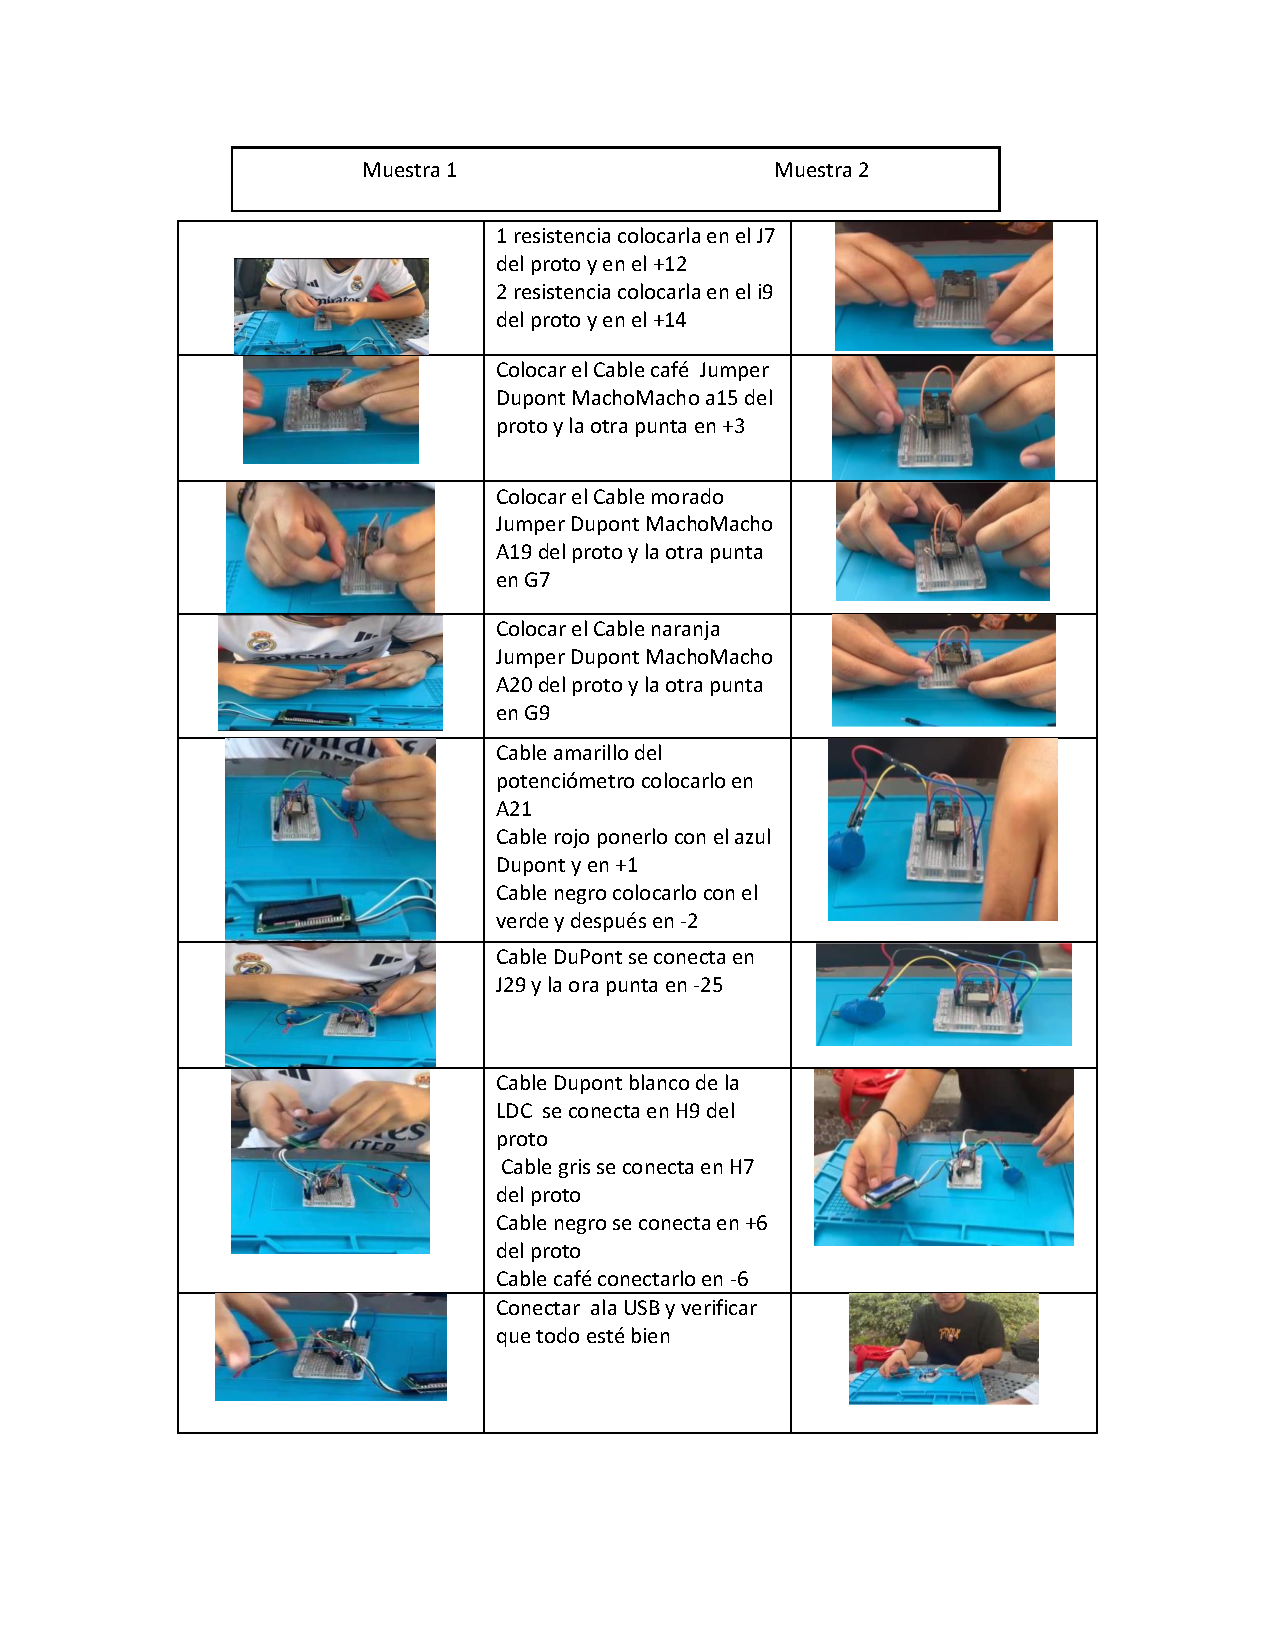
\includegraphics[trim = {10mm 20mm 10mm 8mm},clip,scale=0.45]{29/manual.pdf}
        \caption{muestra los pasos que se siguieron para dicho ensamble }
        \label{fig:manual.pdf}
    \end{figure}
    % 
    % 
    % 
    \subsection{Desarrollo de la guía de plan de Emergencia}
    
    El Plan de Emergencia: documento detallado que describe los procedimientos y acciones a seguir en caso de que ocurra un evento inesperado. Sirve para garantizar la seguridad y el bienestar de las personas, así como para proteger los activos y la infraestructura de la institución así  como estrategias preventivas y correctivas a seguir para garantizar la continuidad operativa del servicio.
    % 
    % 
    \subsection{Análisis de los métodos, materiales, herramientas e instalación utilizada en la ejecución del ensamble de un circuito electrónico}
    
    \subsubsection{Planeación}
    
    Asegúrate de conocer siempre tu objetivo.
    Asegúrate de contar con los documentos (formatos, procedimientos, etc).
    % 
    % 
    \subsubsection{5's}
    
    Las etapas son las siguientes: Seleccionar:Consiste en identificar y clasificar los materiales indispensables para la ejecución del ensamble. El resto, se considerará material innecesario y por lo tanto se eliminará o separará.
    Ordenar: se procede a ordenar los materiales indispensables, facilitando las tareas de encontrar, usar y reponer estos útiles, Con ello se consigue eliminar tiempos no productivos.
    Limpiar: se debe mantener ordenado todo el espacio donde se esta trabajando reduciendo  en gran medida los accidentes y lesiones.
    Estandarizar: el personal debe ser capaz de discernir cuando las tres eses anteriores se están aplicando correctamente y cuando no.
    Sostener: se debe de disponer de una disciplina para mantener un puesto de trabajo ordenado y limpio.
    % 
    % 
    \subsubsection{Desarrollo del sistema de tiempos predeterminado}
    El sistema de tiempos predeterminados (STP) se basa en una metodología  utilizada en ingeniería industrial y gestión de operaciones para estimar el tiempo necesario para llevar a cabo una tarea específica. Este sistema se basa en una serie de movimientos predefinidos y cronometrados que un trabajador realiza para completar una tarea estándar. este sistema se basa en 17 Therblings se centran en los movimientos del operario con el fin de reducir el numero tareas a realizar desde el comienzo de un proceso  hasta finalizar.
    \begin{figure}[H]
        \centering
        \includegraphics[trim = {20mm 82mm 20mm 25mm},clip,scale=0.45]{29/img/therblingsDieciete.pdf}
        \caption{17 Therblings }
        \label{fig:therblingsDieciete.pdf}
    \end{figure}
    A partir de estos Therbligs se desarrollaron diversos sistemas que pueden ser más o menos precisos, más fáciles de aplicar, más consistentes o más adecuados para una industria especifica. El MTM-1 es el sistema que emplearemos a lo largo del proyecto. El MTM-1 es un sistema de medición de tiempos que descompone las actividades de trabajo en elementos básicos para establecer estándares de tiempo en entornos industriales y de fabricación.
    
    Movimientos MTM-1:
    1. Alcanzar: se refiere a un movimiento específico que implica extender el brazo para agarrar o manipular un objeto. (vease en la figura 3)
    
    2. Mover: implica desplazar un objeto de una ubicación a otra.( vease en la figura 5)
    
    3. Girar y Aplicar presión: se utilizan para descomponer las tareas en elementos básicos y calcular el tiempo requerido para realizar esas tareas de manera eficiente.
    
    4. Asir: implica tomar un objeto con la mano o las manos.
    
    5. Colocar en Posición: implica colocar un objeto en una posición específica y orientada de manera adecuada para realizar una tarea determinada.
    
    6. Soltar: implica liberar un objeto que se está sujetando o manipulando, y se utiliza para descomponer las tareas en elementos básicos y calcular el tiempo necesario para realizar esas tareas de manera eficiente.
    
    7. Desenganchar: implica separar o liberar dos objetos que están conectados entre sí.
    
    9. Movimientos del cuerpo (Pierna-Pie, horizontal y vertical): Los movimientos se realizan con todo el cuerpo.
    
    10. Movimientos Simultáneos: acciones realizadas al mismo tiempo con diferentes partes del cuerpo o con diferentes objetos.
    \begin{figure}[H]
        \centering
        \includegraphics[trim = {20mm 82mm 20mm 25mm},clip,scale=0.9]{29/img/alcanzarRa.pdf}
        \caption{Valores estándar del Therbligs Alcanzar.}
        \label{fig:alcanzarRa.pdf}
    \end{figure}
    
    \begin{figure}[H]
        \centering
        \includegraphics[trim = {20mm 82mm 20mm 25mm},clip,scale=0.9]{29/img/Tmu.pdf}
        \caption{Unidades de Medida De Tiempo}
        \label{fig:Tmu.pdf}
    \end{figure}
    
    \begin{itemize}
        \item Literal: Sigla o inicial de la palabra del idioma
    ingles que significa el movimiento fundamental.
    \item Distancia: Camino que sigue el nudillo o la punta
    del dedo a la distancia en l´ınea recta entre los dos
    puntos.
    \item Caso: Situación en la que se realice la operación.
    \end{itemize}
    \begin{figure}[H]
        \centering
        \includegraphics[trim = {20mm 82mm 20mm 25mm},clip,scale=0.9]{29/img/moverM.pdf}
        \caption{Valores estándar del Therbligs Mover}
        \label{fig:moverM.pdf}
    \end{figure}
    Por otro lado, la celda resultante de la intersección
    de la distancia y caso seleccionado, determinara el valor
    estándar del TMU.
    \begin{figure}[H]
        \centering
        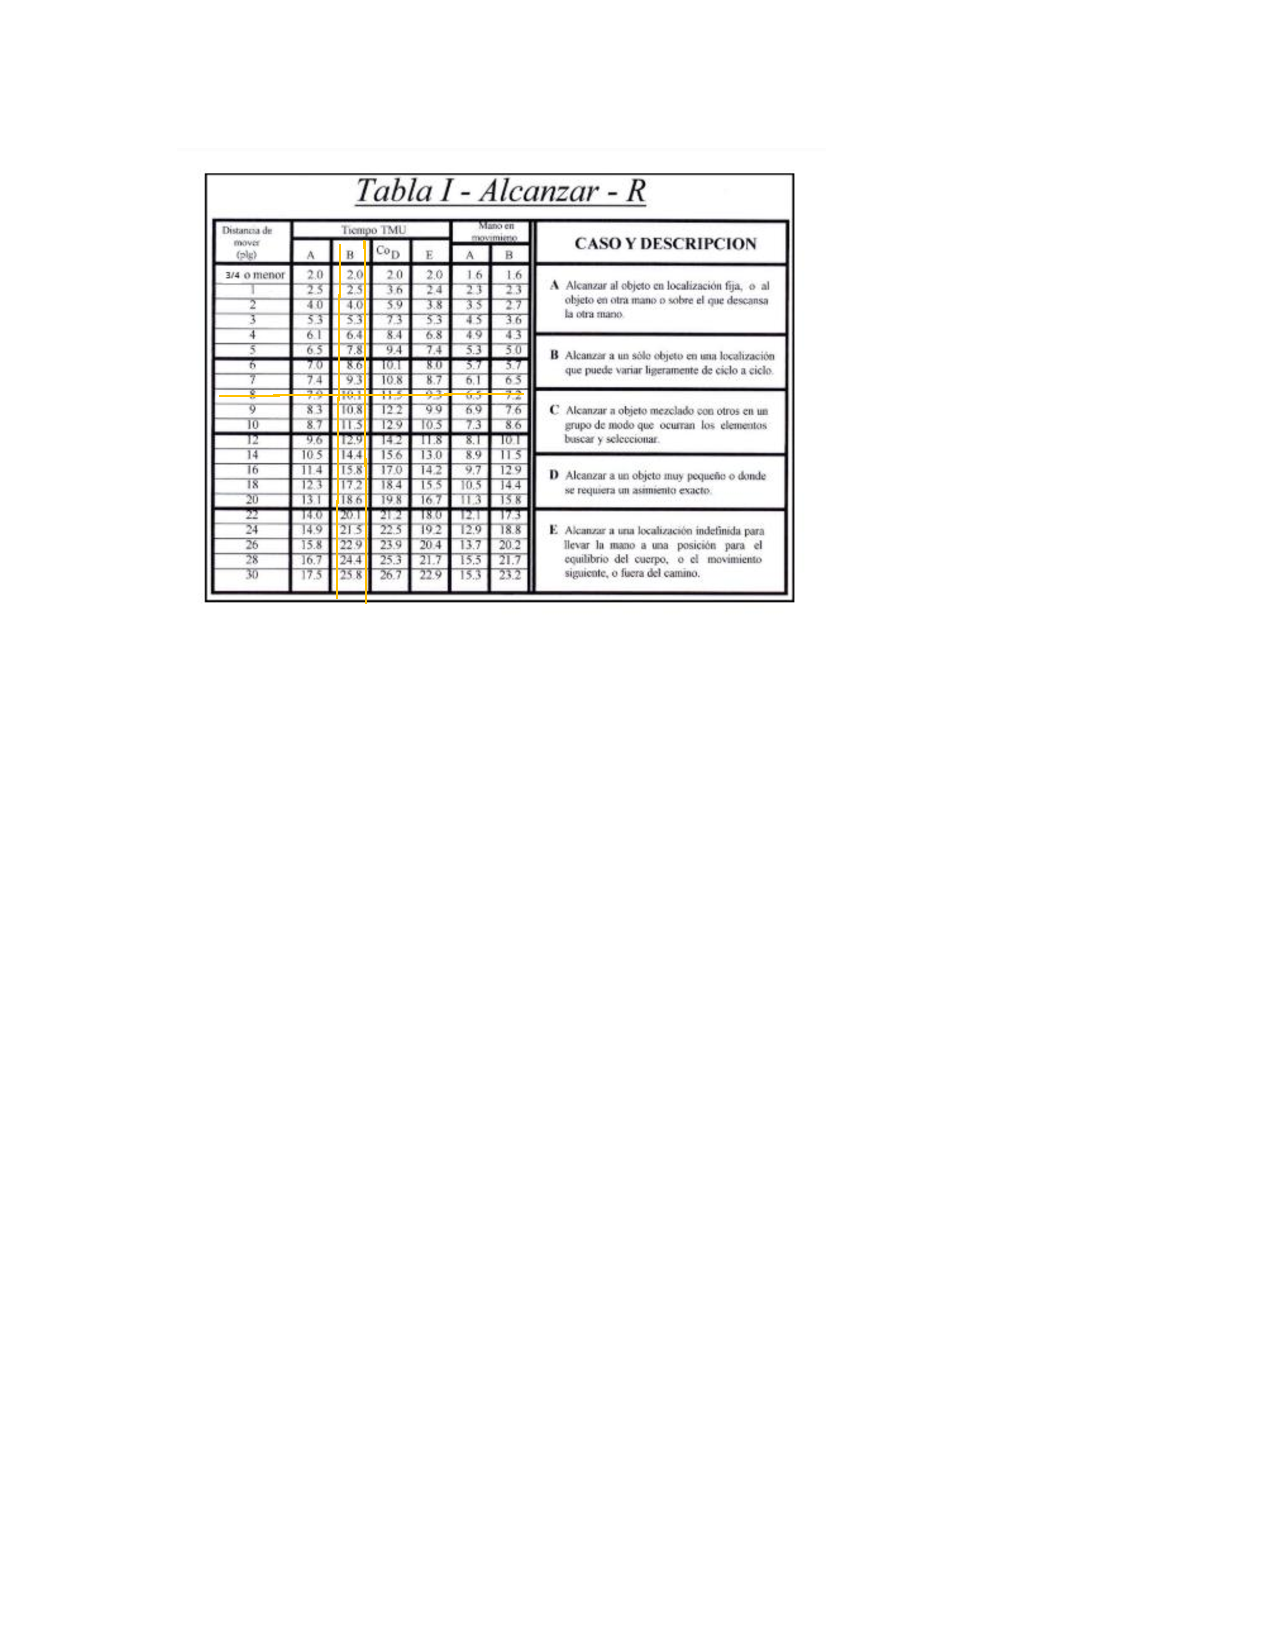
\includegraphics[trim = {20mm 82mm 20mm 25mm},clip,scale=0.9]{29/img/tablaTmu.pdf}
        \caption{Para alcanzar un objeto va  variar su
    ubicación de ciclo a ciclo que se encuentra a una
    distancia de 8 pulgadas se codifica de la siguiente
    manera R8B = 10.1 TMU.}
        \label{fig:tablaTmu.pdf}
    \end{figure}
    % 
    % 
    \subsubsection{Desarrollo del muestreo del trabajo}
    El muestreo del trabajo es un proceso integral dentro del campo de la ingeniería industrial y la gestión de operaciones, diseñado para estudiar y analizar sistemáticamente la forma en que se realizan las tareas en un entorno de trabajo específico. Este enfoque se centra en recopilar datos precisos y representativos sobre el tiempo y el método utilizado para llevar a cabo una tarea, con el objetivo de comprender mejor los procesos, identificar áreas de mejora y establecer estándares de rendimiento.
    % 
    % 
    \subsubsection{Corrección por balanceo de procesos}
     La corrección por balanceo de proceso es importante  para optimizar la eficiencia operativa y maximizar la productividad en entornos de fabricación y producción. Al equilibrar adecuadamente la carga de trabajo, las organizaciones pueden reducir los tiempos de espera, minimizar los cuellos de botella y mejorar la utilización de los recursos, lo que conduce a una mayor eficiencia, menor desperdicio y costos reducidos.Metodología utilizada en la gestión de operaciones y la ingeniería industrial para optimizar la eficiencia y la productividad de los procesos de fabricación, ensamblaje o cualquier operación que involucre una secuencia de tareas o actividades.
    % 
    % 
    \subsubsection{Datos estándar continuos y discretos}
    Los datos estándar continuos son mediciones continuas o variables recopiladas en el circuito electrónico, producción u operación, que se utilizan para monitorear, controlar y mejorar el rendimiento del proceso y la calidad del producto.
    % 
    % 
    \subsection{Diseño de la forma más económica de realizar el trabajo}
     El diseño de la forma mas económica de realizar el trabajo Se enfoca en el  desarrollo del  proceso que maximice la eficiencia. Esto implica analizar todos los aspectos del ensamblaje, desde la utilización de recursos hasta la optimización del  proceso, con el objetivo de lograr los mejores resultados. Esto puede implicar la optimización de la utilización de materiales, la reducción de los tiempos, la mejora de la logística, se trata de encontrar la mejor manera de realizar dicho ensamble en términos de costos de materiales y recursos utilizados.
    
    % 
    % 
    \subsection{Normalización de los métodos, materiales, herramientas e instalaciones}
    La normalización de los métodos, materiales, herramientas e instalaciones es elemental dentro de este proyecto ya que  favorece al  proceso integral que contribuye a mejorar la eficiencia, la calidad y la seguridad en el área de trabajo 
    así también  garantiza la compatibilidad y el correcto funcionamiento de los componentes electrónicos y  reduce costos al minimizar errores. Además, establece pautas claras para la selección de materiales, el uso de herramientas específicas y la configuración de instalaciones. Al adherirse a normas establecidas, se fomenta la innovación y se facilita la integración de nuevas tecnologías en el diseño y fabricación de circuitos electrónicos. En cuanto a los materiales utilizados en el proyecto, se menciona que son indispensables para alcanzar los objetivos deseados y se presenta una lista detallada de los mismos.
    \begin{figure}[H]
        \centering
        \includegraphics[trim = {10mm 20mm 10mm 8mm},clip,scale=0.30]{29/img/listaDm.pdf}
        \caption{Lista de materiales con las cantidades utilizadas  }
        \label{fig:listaDm.pdf}
    \end{figure}
    % 
    % 
    \subsection{Determinación del tiempo estándar para que una persona competente realice el trabajo con marcha normal}
    D.1. LCD de 16x2 es es un tipo de pantalla de cristal líquido (LCD) que tiene la capacidad de mostrar hasta 16 caracteres por línea y cuenta con 2 líneas de visualización que muestran el  texto, símbolos y gráficos simples de una manera legible y fácil de entender. Son controladas por un microcontrolador o un circuito integrado dedicado y pueden mostrar una variedad de información.
    D.2. Protoboard 400 puntos es una herramienta fundamental en la creación de prototipos electrónicos. Se trata de una placa de circuito impreso (PCB) con orificios y conexiones metálicas que permiten insertar y conectar componentes electrónicos de manera temporal para crear circuitos experimentales sin necesidad de soldadura.
    
    Tipo: Protoboard
    Puntos: 400 puntos
    Color: Transparente
    Material: Plástico (ABS)
    Longitud: 80 mm
    Ancho: 51 mm
    Altura: 8.3 mm
    Peso de la unidad: 40 g
    Voltaje m´máximo: 36 V
    Máxima capacidad de corriente: 3A
    Acepta cables con diámetro: 0.2 a 0.7 mm
    
    % 
    % 
    % \subsection{Acrónimos y Abreviaciones}
    
    % Los acrónimos y abreviaciones deberán ser definidos únicamente la primera vez que aparecen en el texto, esto para que el lector entienda lo que significan.
    
    % \subsection{Ecuaciones}
    
    % Las ecuaciones son una excepción a las especificaciones prescritas de esta plantilla. 
    % Deberá determinar si su ecuación debe escribirse o no utilizando la fuente Adobe Devangari. 
    % Para crear ecuaciones multinivel, puede ser necesario tratar la ecuación como un gráfico e insertarla en el texto después de aplicar el estilo de la platilla.
    % Las ecuaciones serán enumeradas de manera consecutiva, y el número de ecuación, entre paréntesis, se colocan al ras de la derecha, utilizando una tabulación derecha.
    % 
    % \begin{equation}
    %     \label{eq1}
    %     x + y = z 
    % \end{equation}
    % 
    % Es importante asegurarse de que los símbolos de la ecuación sean definidos antes o inmediatamente después de la ecuación. Utilice “(1)”, en vez de “Eq. 1” al enumerar las ecuaciones, excepto al principio de una oración: “La ecuación (\ref{eq1}) es…”
    
    \section{Resultados y discusión}
    
    \subsection{Desarrollo de la guía de plan de Emergencia}
    
    Con esta guía buscamos analizar, identificar y evaluar los posibles accidentes internos y externos dentro del instituto Tecnológico de Queretaro , capacitando al personal en un tiempo establecido para salvaguardar la integridad.
    
    % 
    % 
    \begin{figure}[H]
        \centering
        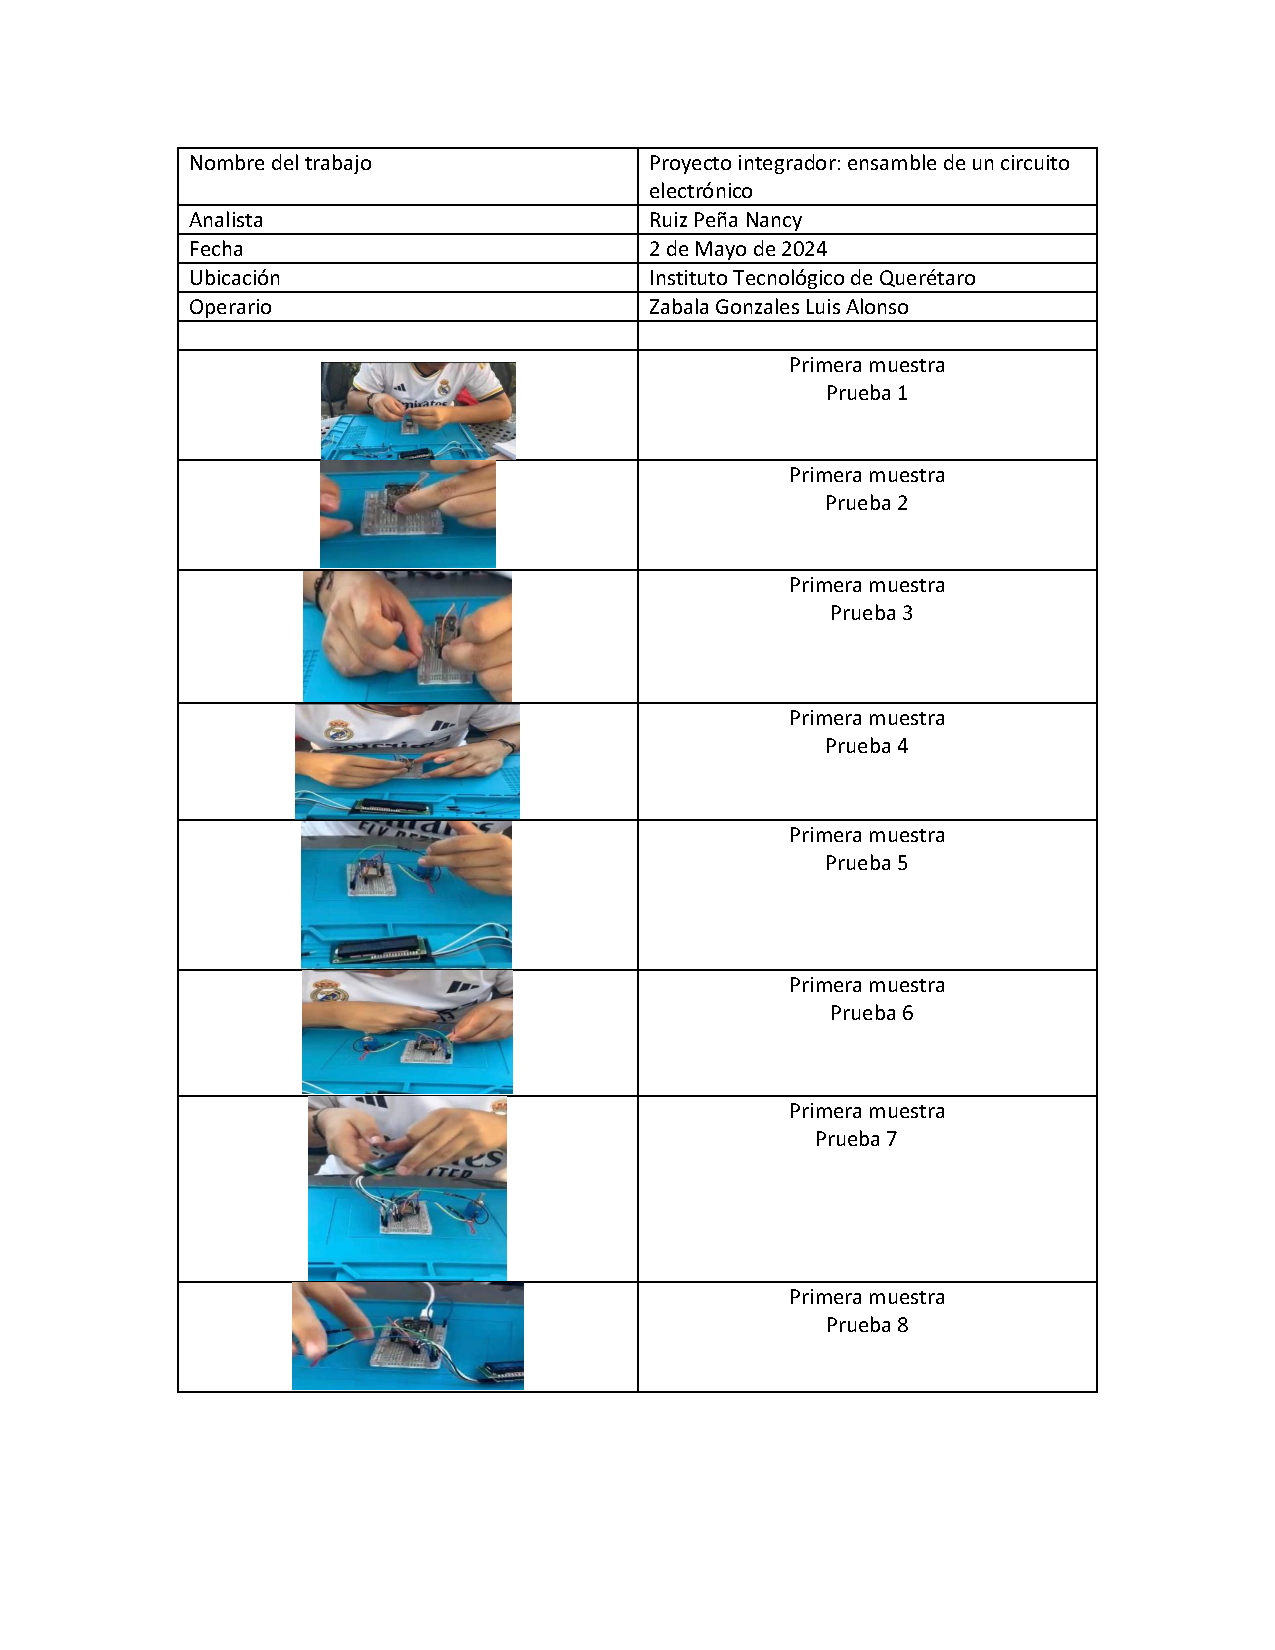
\includegraphics[scale=0.40]{29/img/hojaRegistros.pdf}
        \caption{Hoja de registro 1 }
        \label{fig:hojaRegistros.pdf}
    \end{figure}
    
    En la siguiente tabla se muestran los resultados de la segunda muestra
    \begin{figure}[H]
        \centering
        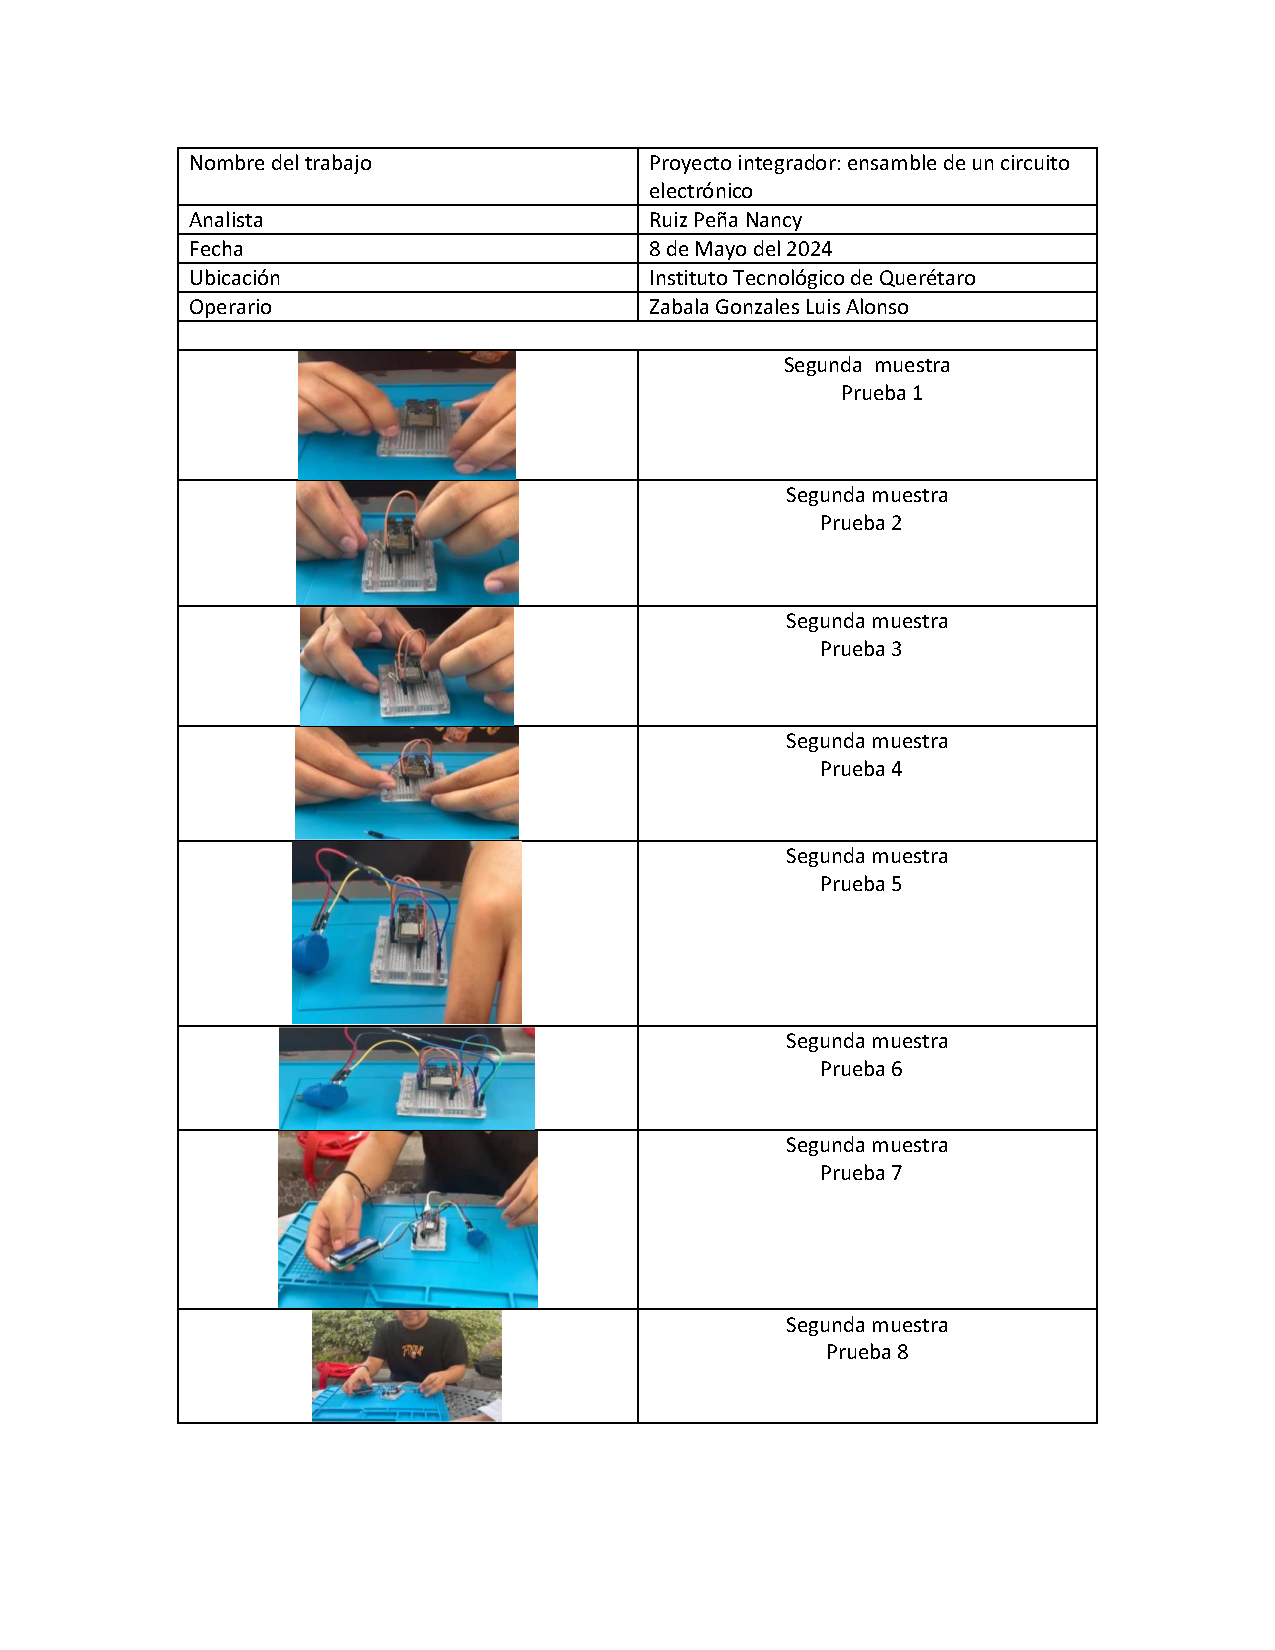
\includegraphics[scale=0.40]{29/hojasRegistro.pdf}
        \caption{Hoja de registro 2 }
        \label{fig:hojasRegistro.pdf}
    \end{figure}
    se presentan las dos muestras con la lectura 1 y 2 con dicho calculo 
    \begin{figure}[H]
        \centering
        \includegraphics[scale=0.40]{29/registroLecturas.pdf}
        \caption{Hoja de registro de las lecturas, parte 1  }
        \label{fig:registroLecturas.pdf}
    \end{figure}
    
    \begin{figure}[H]
        \centering
        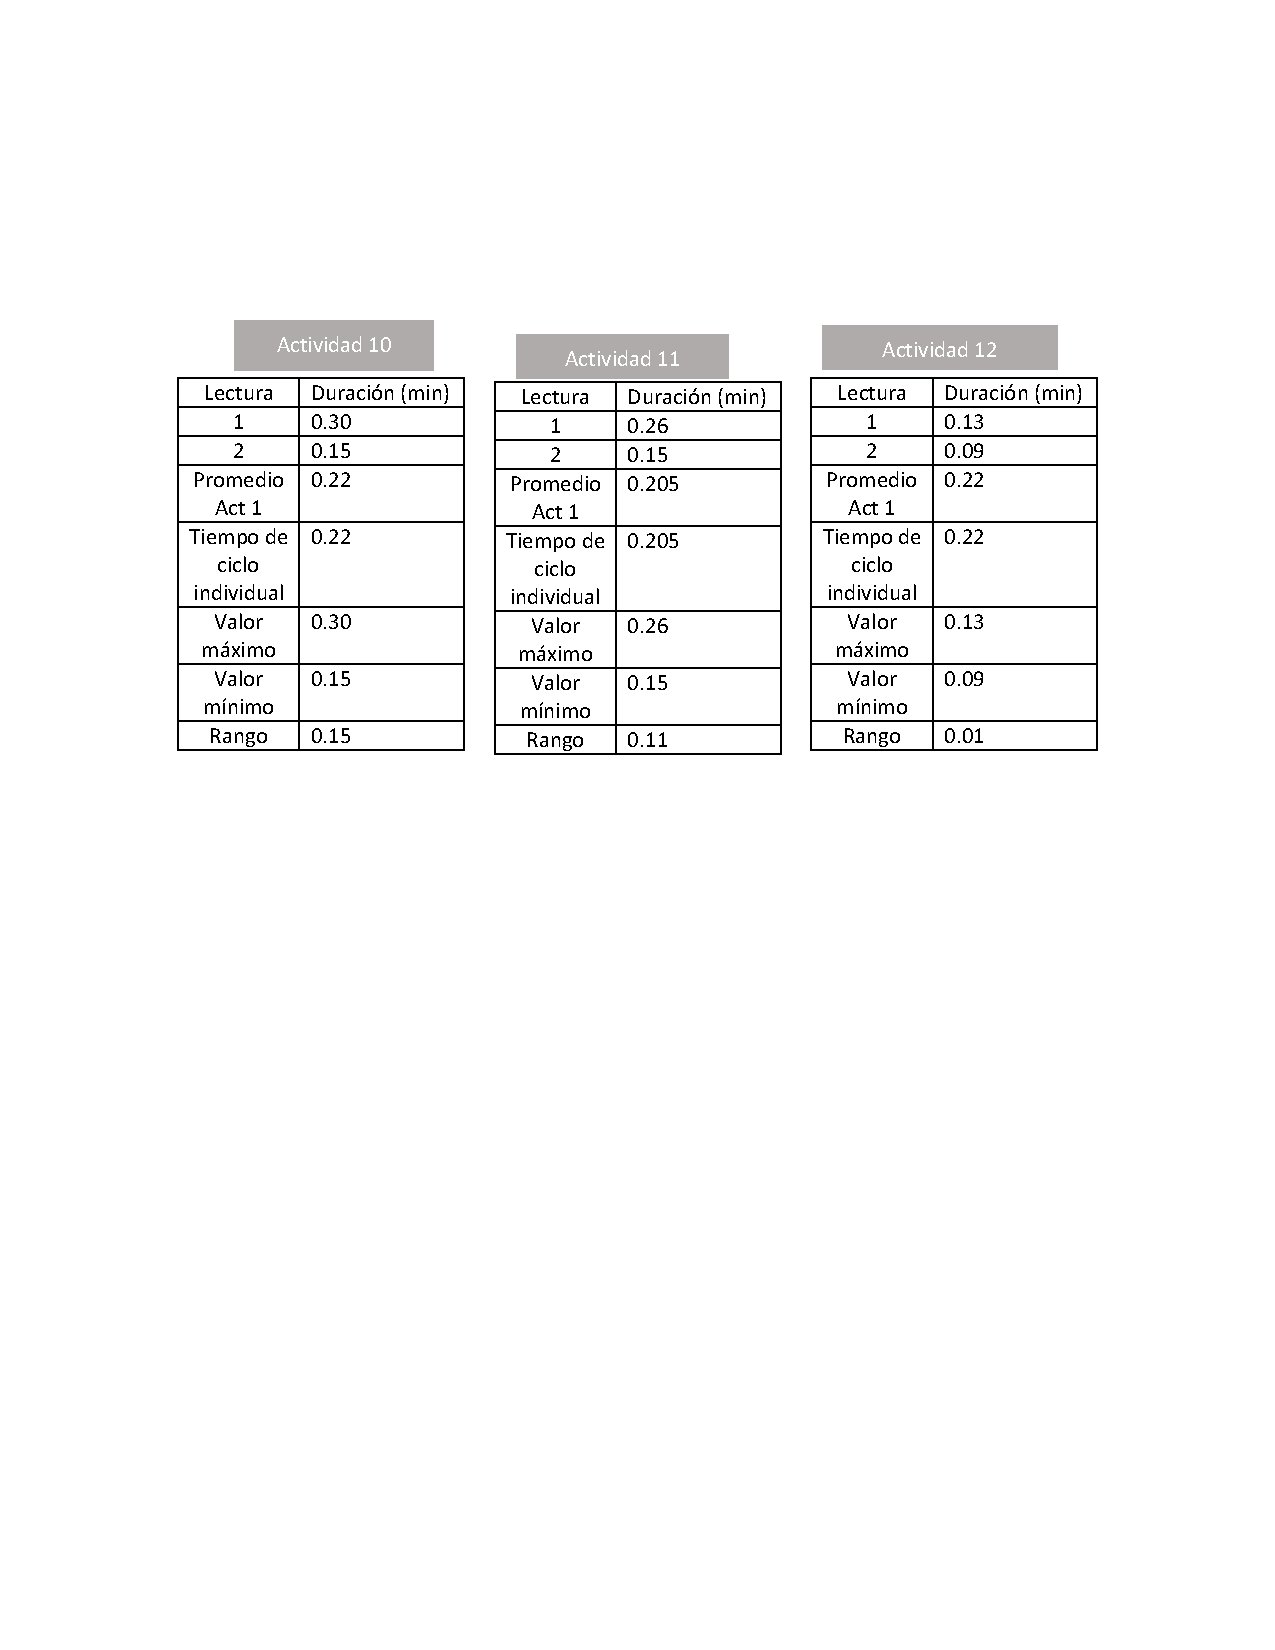
\includegraphics[scale=0.40]{29/registrosLectura.pdf}
        \caption{Hoja de registro de las lecturas, parte 2  }
        \label{fig:registrosLectura.pdf}
    \end{figure}
    
    % 
    % 
    \subsubsection{Identificación del riesgo}
    
    Estamos comprometidos a mantener todos los días un programa interno de prevención de riesgos, así como una retroalimentación por parte de clientes internos y externos en los riesgos que se presentan en las actividades constantes por su parte invitamos a utilizar el equipo de trabajo, permitiendo anticiparnos a posibles problemas, proteger nuestros recursos, mejorar la toma de decisiones y  optimizar el uso de nuestros recursos , cumplir con las regulaciones aplicables lo que Implica identificar posibles amenazas como incendios, accidentes, intrusiones,  eventos climáticos extremos.
    Evaluamos a cada riesgo interno por un rango para dar prioridad en las acciones 
    
    
    % 
    % 
    \subsubsection{Riesgos internos}
    
    El riesgo se define como la posibilidad de que algo suceda o no suceda en otras palabras es la proximidad de un daño. 
    El riesgo operativo interno lo definimos como la posibilidad de que sufre la empresa derivado de los fallos naturales en su propio funcionamiento refiriéndose a los peligros, amenazas o potenciales problemas que pueden surgir dentro de un proceso o sistema laboral y que son generados o controlados por factores internos de la organización. Estos riesgos están relacionados con aspectos como la organización del trabajo, la gestión de recursos humanos, la eficiencia operativa y la seguridad en el lugar de trabajo
    % 
    % 
    \begin{table}[h]
        \centering
        \caption{Riesgos con diferentes niveles y colores para distinguir la gravedad y acciones}
        \begin{tabular}{c c c}
        \hline
        \multicolumn{3}{c}{Riesgos}\\
        \hline
             Alto& 0.99 - 0.18 & Rojo  \\
        \hline
             Medio& 0.17 - 0.05 & Amarillo  \\
        \hline
             Bajo& 0.04 - 0.01 & Verde \\
        \hline     
        \end{tabular}
        \label{tab:riego}
    \end{table}
    % 
    % 
    % \begin{table}[h]
    %     \centering
    %     \caption{Descripción de los riesgos al realizar las actividades más comunes y de riesgo dentro de la empresa}
    %     \begin{tabular}{|c|c|c|c|p{7em}|c|}
    %          \hline
    %          Causa& Descripción del riesgo& Probabilidad& Impacto& Acciones Preventivas& Responsable \\
    %          \hline
    %          Gestión& Herida lacerada& 0.01 Bajo& Muy bajo& No utilizar navaja solo cúter&  \\
    %          \hline
    %          Gestión& Golpe con martillo& 0.01 Bajo& Muy bajo& Capacitación&  \\
    %          \hline
    %          Gestión& Levantar super sacos& 0.17 Medio& bajo& Utilizar faja y recibir ayuda&  \\
    %          \hline
    %          Gestión& Carga de camionetas& 0.01 Bajo& Muy bajo& Utilizar faja y guantes&  \\
    %          \hline
    %          Cliente& Descarga de camioneta& 0.17 medio& bajo& Utilizar faja y guantes&  \\
    %          \hline
    %          Gestión& Corto circuito& 0.17 medio& bajo& Revisar las conexiones de la fuente de energía cada mes&  \\
    %          \hline
    %          Cliente& Fumador& 0.01 Bajo& Muy bajo& Señalamientos y llamada de atención&  \\
    %          \hline
    %     \end{tabular}
    %     \label{tab:Riesgos}
    % \end{table}
    % 
    % 
    \begin{figure}[H]
        \centering
        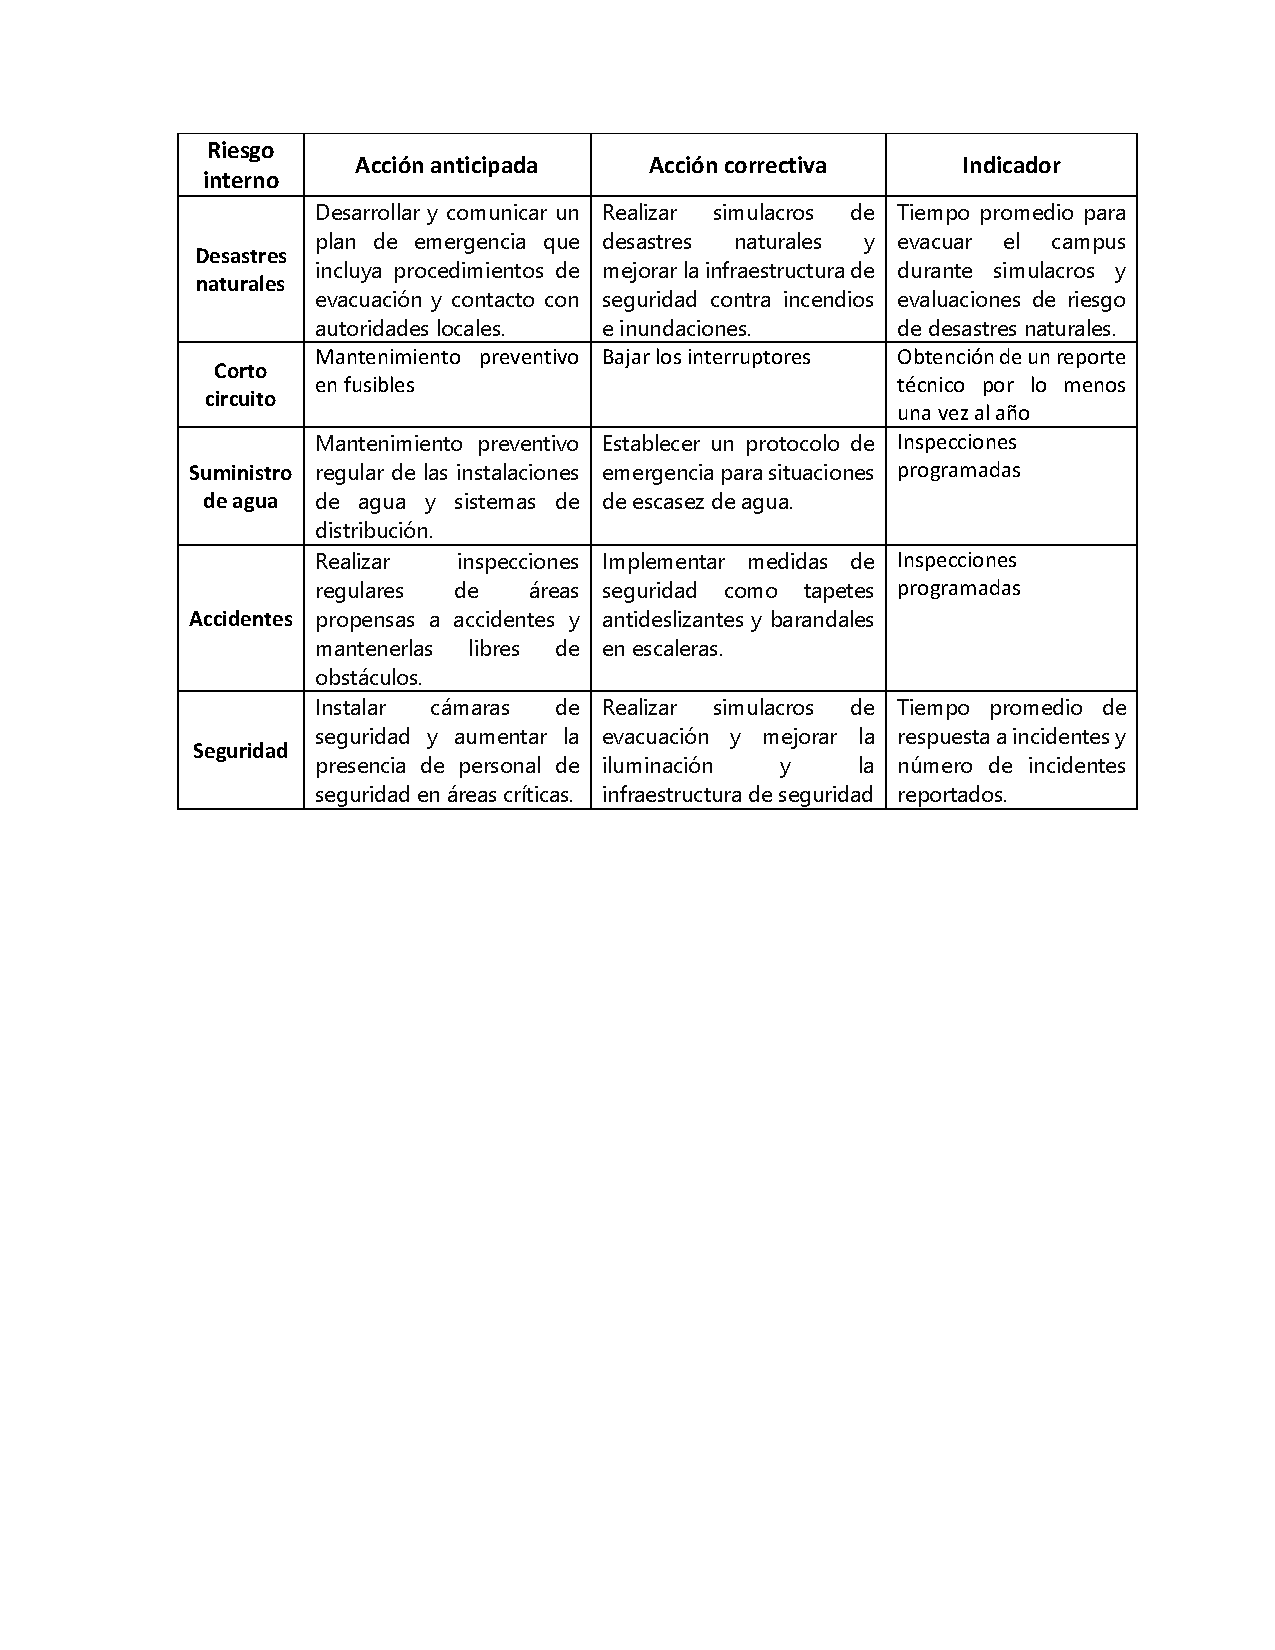
\includegraphics[trim = {20mm 130mm 20mm 20mm},clip,scale=0.45]{29/img/riesgoInterno.pdf}
        \caption{Descripción de los riesgos al realizar las actividades más comunes y de riesgo dentro de la empresa}
        % \label{fig:riesgoInterno.pdf}
    \end{figure}
    % 
    % 
    \subsubsection{Riesgos externos}
     en cambio los riesgos externos se refieren a cualquier amenaza o peligro que proviene del entorno externo de una organización y que puede afectar negativamente a sus operaciones, objetivos o resultados son inherentemente difíciles de predecir y controlar, ya que están fuera del control directo de la organización o individuo afectado.
     Mencionamos las diferentes acciones de lo que se piensa hacer cuando ocurra un riesgo interno o externo haciendo anticipadamente las actividades de la institución para evitar riesgos 
    % \begin{table}[H]
    %     \centering
    %     \caption{Descripción de los riesgos externos}
    %     \begin{tabular}{|c|c|c|p{10em}|}
    %          \hline
    %          Descripción del riesgo& Probabilidad& Impacto& Acciones preventivas\\
    %          \hline
    %          Desmayo del cliente& 0.01 bajo& Muy bajo& Colocar al cliente en una posición apropiada para la llegada de los paramedicos\\
    %          \hline
    %          Incendio de algún vecino& 0.01 bajo& Alto& Mantener los detectores de humo en lugares estratégicos y con pilas\\
    %          \hline
    %          Incendio de camioneta& 0.17 moderado& Alto& Mantener en mantenimiento los sensores de temperatura y con un extintor \\
    %          \hline
    %          Incendio por pirotecnia& 0.17& Alto& Vigilar en los días festivos y mojar el material\\
    %          \hline
    %          Choque en la avenida& 0.17& Medio& Delimitar y poner conos de señalamiento\\
    %          \hline
    %     \end{tabular}
    %     \label{tab:RiesgosExternos}
    % \end{table}
    % 
    % 
    \begin{figure}[H]
        \centering
        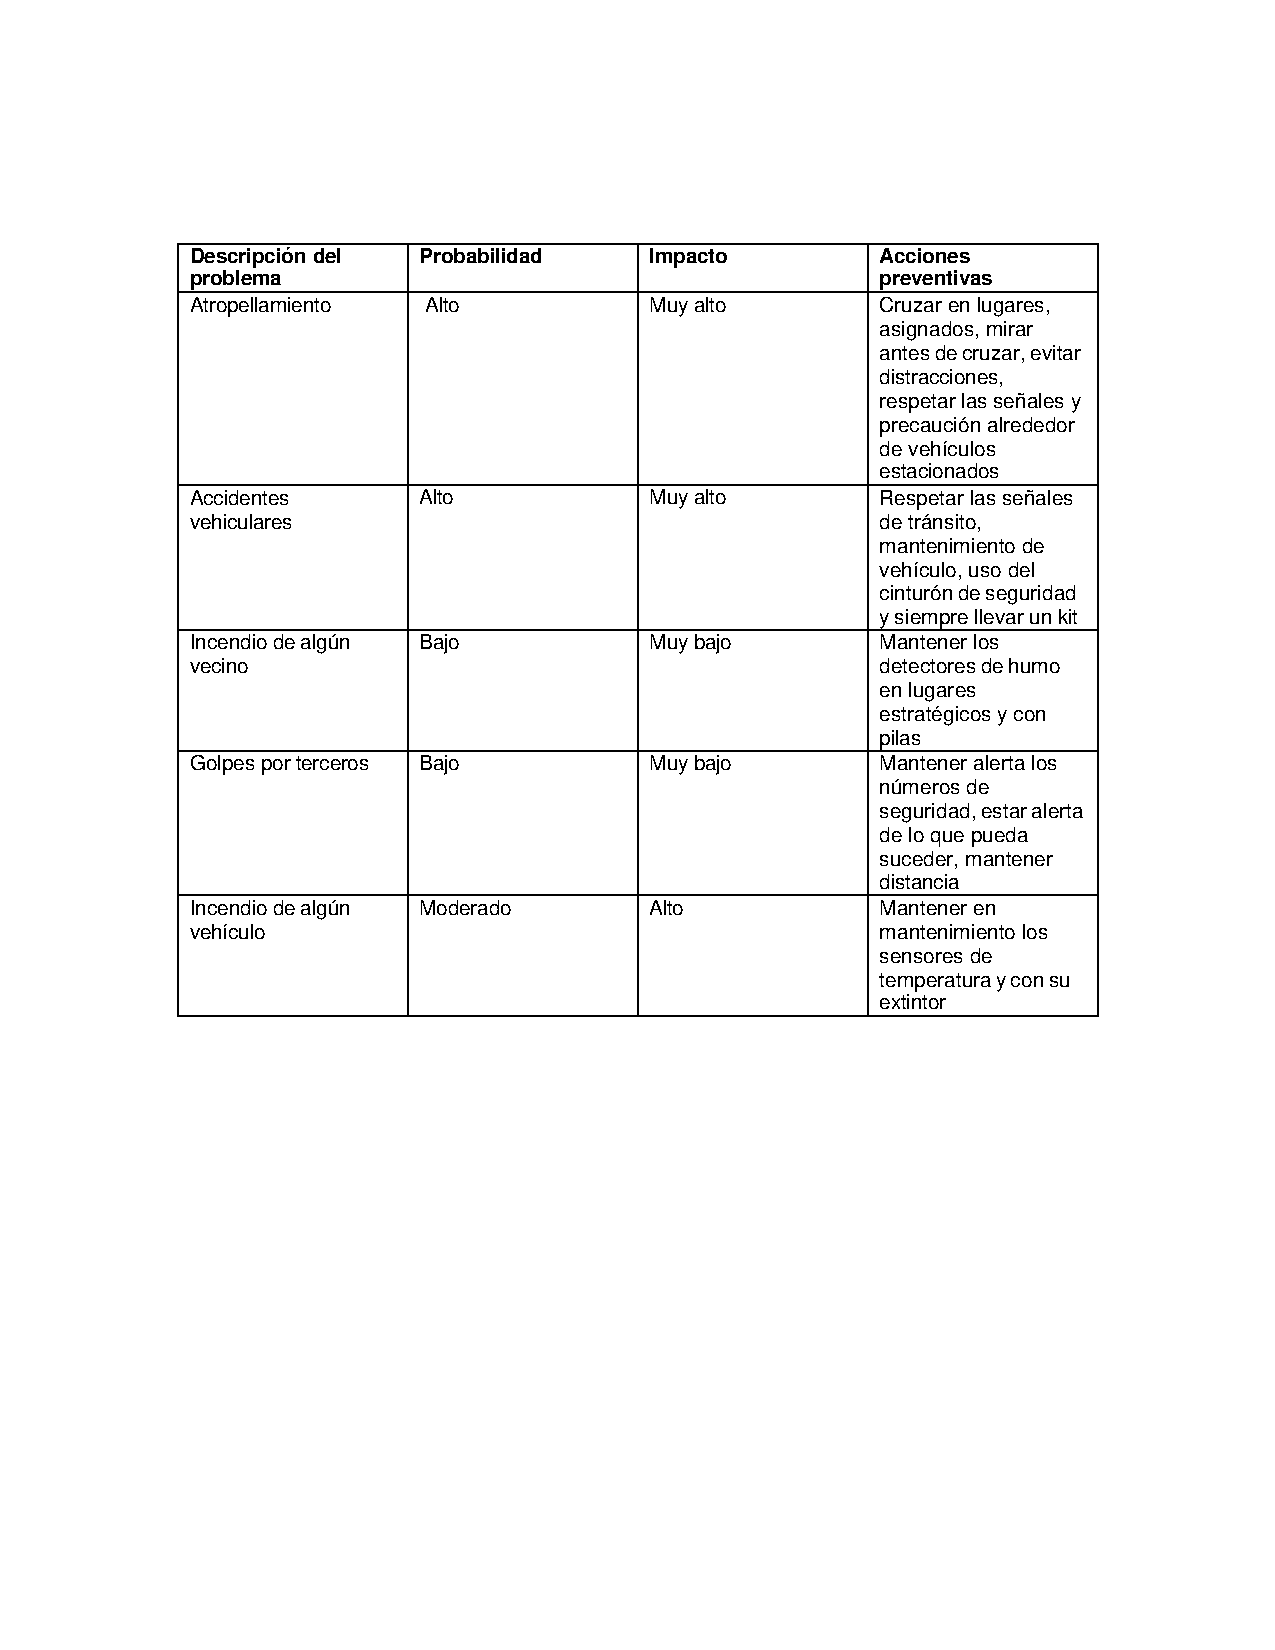
\includegraphics[trim = {10mm 90mm 10mm 10mm},clip,scale=0.5]{29/img/riesgoExternos.pdf}
        \caption{Descripción de los riesgos externos}
        \label{fig:riesgoExternos.pdff}
    \end{figure}
    % 
    % 
    \subsubsection{Programa de actividades de prevención y auxilio}
    se plantea en base al  conjunto organizado de acciones diseñadas para prevenir y responder efectivamente a situaciones de emergencia o desastres .Las actividades de preparación y disposición que se hace anticipadamente en el ITP para evitar riesgos.
    % 
    % 
    \subsubsection{Plan de acción}
    
    este plan  establece de manera detallada las medidas específicas que se deben tomar resolver un problema determinado suele incluir una descripción clara de las acciones a realizar, los responsables de llevarlas a cabo, los recursos necesarios, los plazos de ejecución y los criterios de evaluación, además se desarrolla mediante la identificación anticipada de posibles riesgos que pueden ocurrir dentro del ITQ y así garantizar que este preparado para hacer frente en cualquier problema protegiendo la comunidad estudiantil. 
    % 
    % 
    % \begin{table}[H]
    %     \centering
    %     \caption{Descripción de las acciones anticipadas y correctivas ante un riesgo interno}
    %     \begin{tabular}{|p{5em}|p{10em}|p{11em}|p{10em}|}
    %         \hline
    %          RIESGO INTERNO& Acción Anticipada& Acción Correctiva& Indicador\\
    %          \hline
    %          Herida lacerada& Reemplazar las navajas y cuchillos por cutter con resorte. Utilizar en lo menos posible objetos punzo cortantes& Utilizar el material de los primeros auxilios y lavar la herida con agua oxigenada y vendar& Constancias de capacitación así como el registro de la disminución en el uso de curitas\\
    %          \hline
    %          Golpeo con martillo& Capacitación y descansos de 5 minutos cuando se este trabajando constantemente con el martillo& Aplicar pomada para golpes del botiquín de primeros auxilios& Menos reportes de golpes\\
    %          \hline
    %          Levantar super sacos& Capacitar con el uso adecuado de la faja y solicitar ayuda al momento de levantar materiales mayores a 30 kg& Tomar un descanso y tomar agua &Disminución del cansancio al final del día\\
    %          \hline
    %          Carga y descarga de camionetas& Capacitar con el uso adecuado de la faja y solicitar ayuda al momento de levantar materiales mayores a 30 kg& Utilizar más personal para evitar riesgos & Menor tiempo de carga y descarga en la camioneta\\
    %          \hline
    %          Chispa por cigarro& Señalamientos de no fumar a la entrada& Pedir de manera amable que apaguen el cigarro& Observar en el área de trabajo decremento de las colillas de cigarro\\
    %          \hline
    %          Corto circuito& Mantenimiento preventivo en los fusibles en el centro de carga& Bajar los interruptores del centro de carga& Obtención de un reporte técnico por lo menos una vez al año\\
    %          \hline
    %     \end{tabular}
    %     \label{tab:my_label}
    % \end{table}
    % 
    % 
    % \begin{table}[H]
    %     \centering
    %     \caption{Descripción de las acciones anticipadas y correctivas ante un riesgo externo e interno}
    %     \begin{tabular}{|p{5em}|p{10em}|p{11em}|p{10em}|}
    %          \hline
    %          RIESGO EXTERNO& Acción Anticipada& Acción Correctiva& Indicador\\
    %          \hline
    %          Desmayo del cliente& Tomar cursos de primeros auxilios por lo menos una vez al año a todo el personal& Contar con los conocimientos básicos de primeros auxilios& Realizar un simulacro que nos permita evaluar las acciones en el manejo del riesgo por desmayo\\
    %          \hline
    %          Incendio de algún vecino& Mantener los detectores de humo en lugares estratégicos y cambiar las pilas cada 2 meses& Llamar al 911 para informar del incendio y del posible riesgo en el negocio&  Llevar un registro de los cambios de las pilas en los detectores de humo\\
    %          \hline
    %          Incendio de camioneta& Mantener en mantenimiento los sensores de temperatura y con un extintor& Accionar el extintor conforme a lo establecido por el departamento de bomberos y llamar al 911& Revisar el tablero de la camioneta que no indique falta de agua o alta temperatura \\
    %          \hline
    %          Incendio por pirotecnia& Vigilar en los días festivos y mojar el material& Llamar a emergencias y tratar de sofocar el fuego& Hacer un llamado a los vecinos a ser cuidadosos\\
    %          \hline
    %          Choque en la avenida& Delimitar y poner conos de señalamiento& Llamar a emergencias y si es que hay daños a personas, aplicar primeros auxilios en caso de ser necesario& Llevar un registro de las horas pico para evitar hacer maniobras\\
    %          \hline
    %     \end{tabular}
    %     \label{tab:Acciones}
    % \end{table}
    % 
    % 
    \begin{figure}[H]
        \centering
        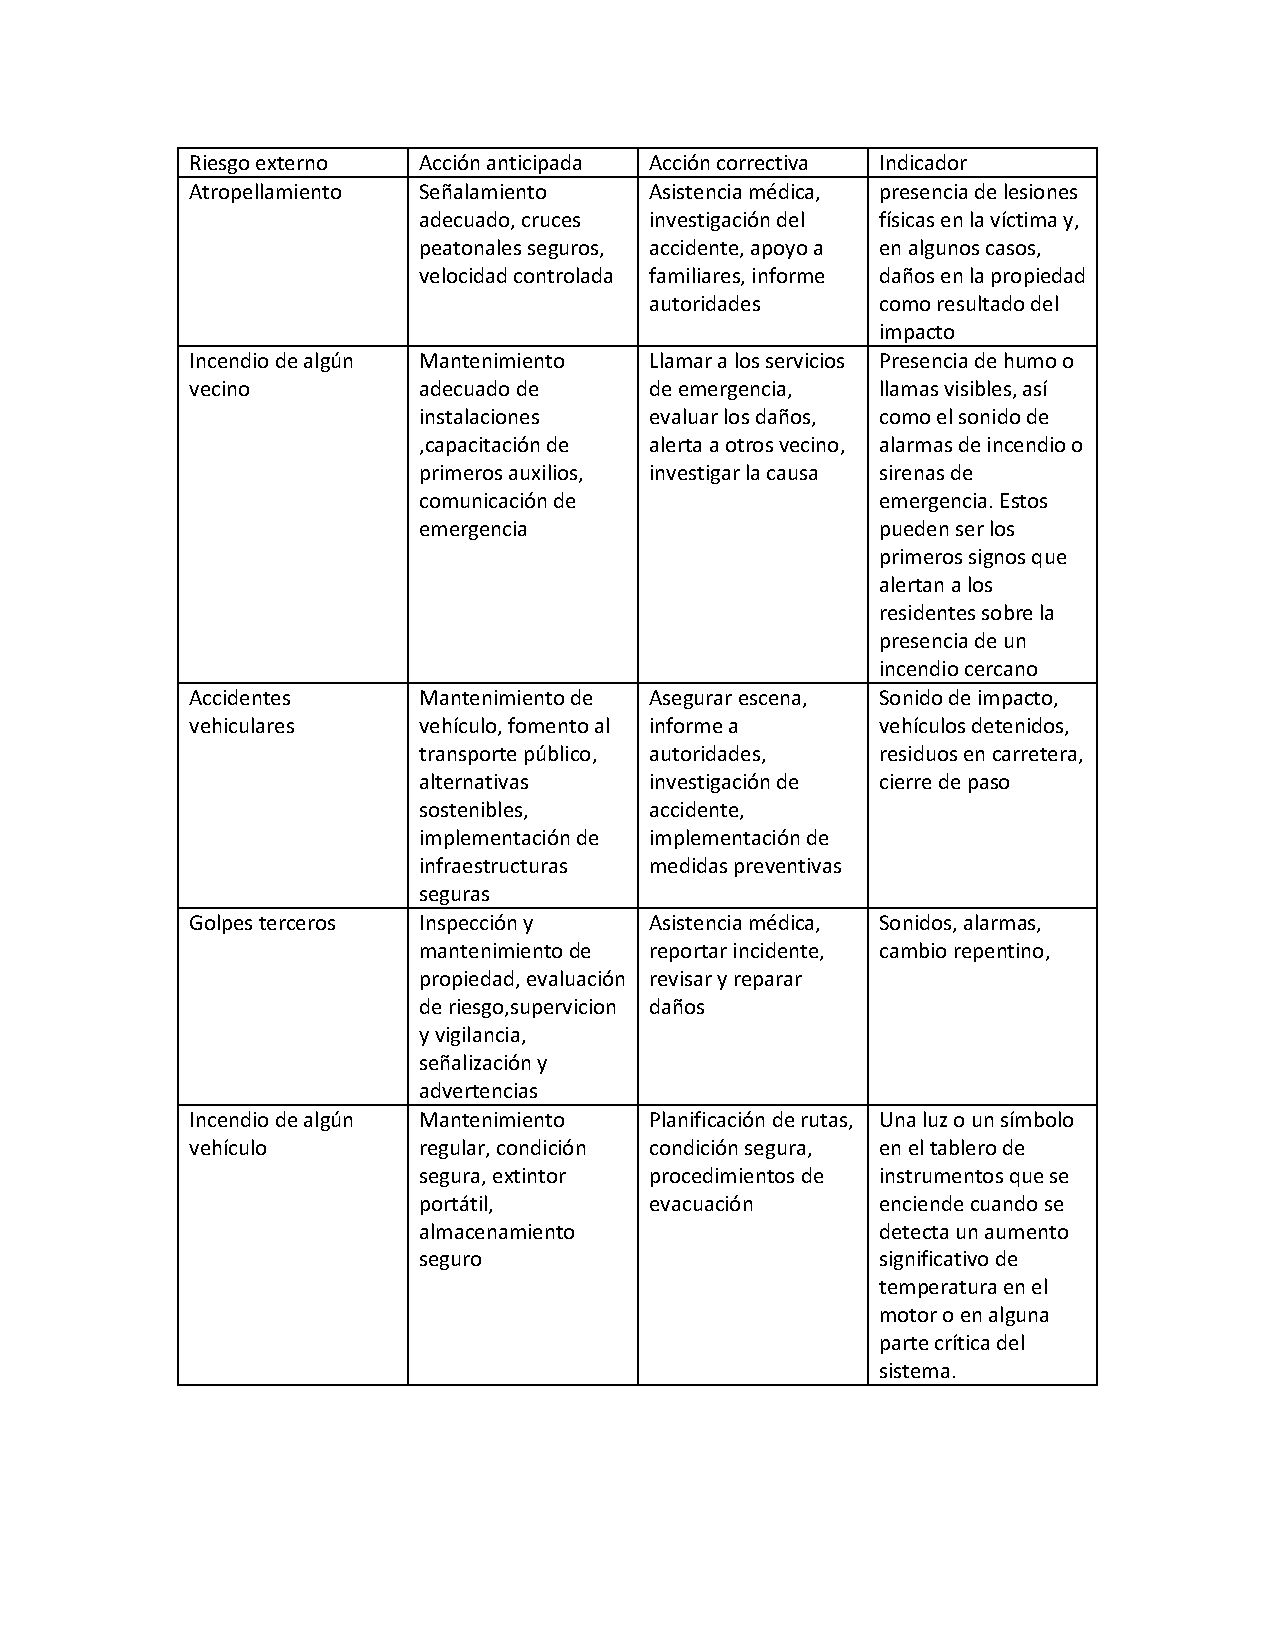
\includegraphics[trim = {20mm 30mm 20mm 15mm},clip,scale=0.45]{29/img/accionesAnticipadas.pdf}
        \caption{Descripción de las acciones anticipadas y correctivas ante un riesgo }
        \label{fig:accionesAnticipadas.pdf}
    \end{figure}
    % 
    % 
    % Cada estrategia metodológica se establece acorde a cada objetivo, y por tanto deberá ser desglosada precisada y ordenada claramente. En consecuencia cada objetivo que se presentó en forma de verbo en infinitivo deberá determinar una estrategia en forma de adverbio. Ej. Desarrollar…Desarrollo. Son las actividades ordenadas que tienen como finalidad la prueba de la hipótesis. 
    
    % \begin{itemize}
    %     \item Se debe establecer que se habrá de hacer, como, conque, y donde para obtener la información que permita probar la hipótesis.  
    %     \item Se debe desglosar de acuerdo a los objetivos específicos. 
    %     \item Se debe establecer una estrategia metodológica por cada objetivo específico. De manera simplista se podría decir que se cambia el verbo en infinitivo por su respectivo adverbio.
    %     \item En cada objetivo se debe describir que método, que materiales y que equipo se usará para conseguirlo.
    %     \item Se deben tener referencias Figura \ref{fig:lcd-16x2}.
    % \end{itemize}
    % 
    % 
    % \begin{figure}[H]
    %     \centering
    %     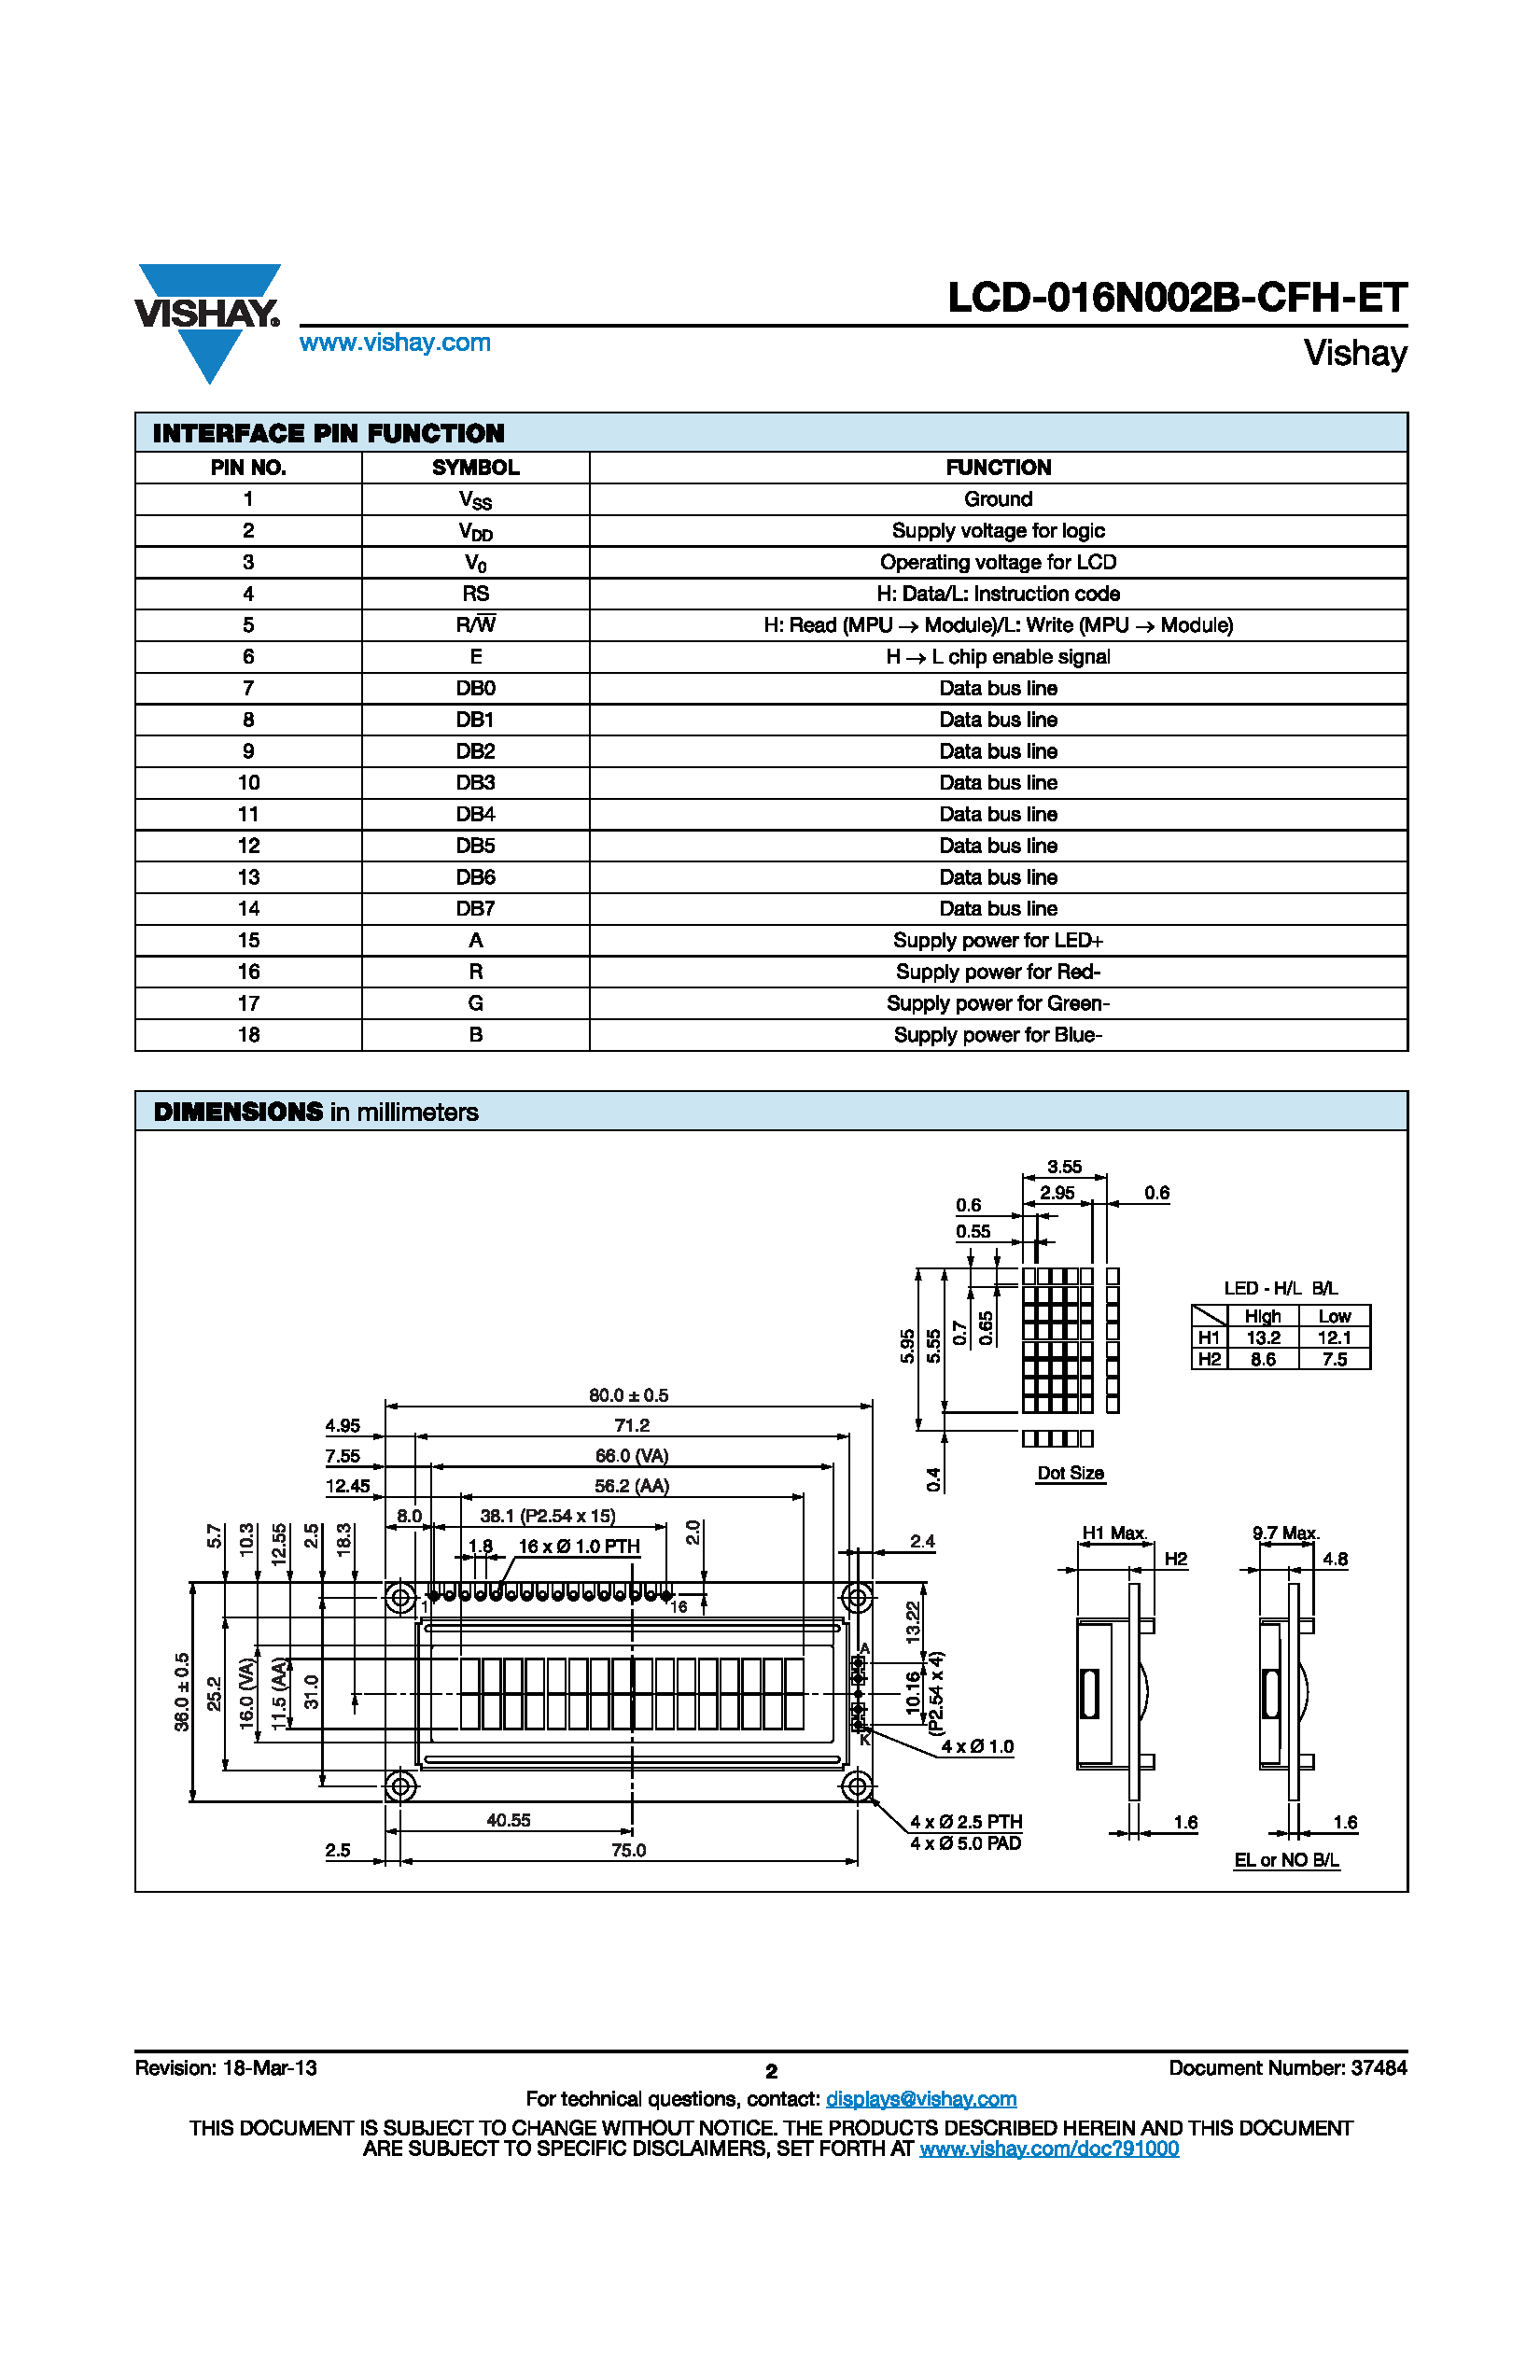
\includegraphics[trim = {30mm 65mm 90mm 250mm},clip,scale=0.5]{6/Img/lcd-16x2.pdf}
    %     \caption{Esquema LCD de 16x2}
    %     \label{fig:lcd-16x2}
    % \end{figure}
    % 
    % 
    % \subsection{Prepara tu documento}
    
    % Antes de que comiences a utilizar esta plantilla, es recomendable que prepare la información que contendrá en un archivo aparte. 
    % Ten preparadas tus gráficas, así como también las tablas aparte, para que sea más fácil integrarlo. 
    % Se recomienda fuertemente el uso de \textbf{formato Enhanced Metafile (.emf) para imágenes y gráficas} de resolución óptima. 
    % Finalmente, completa y organiza el contenido antes de darle el formato de esta plantilla. 
    % 
    % 
    \subsubsection{Identificación de capacidades}
    
    \begin{table}[H]
        \centering
        \caption{Recursos en materia de seguridad}
        \begin{tabular}{c c c}
        \hline
        \multicolumn{3}{c}{Inventario de recursos en materia de seguridad}\\
        \hline
             No.& Recurso & Cantidad  \\
        \hline
             1& Extintor & 8  \\
        \hline
             2& Botiquín & 5 \\
        \hline
             3& Puntos de reunión & 4 \\
        \hline     
        \end{tabular}
        \label{tab:inventario}
    \end{table}
    % 
    % 
    \subsubsection{Plano de localización de recursos}
    
    % 
    % 
    \begin{figure}[H]
        \centering
        \includegraphics[trim = {20mm 25mm 20mm 12mm},clip,scale=0.3]{29/img/planoDelocalizacion.pdf}
        \caption{Plano del establecimiento de los recursos en materia de seguridad.}
        \label{fig:planoDelocalizacion.pdf}
    \end{figure}
    % 
    % 
    \subsubsection{ Identificación de apoyos externos}
    
    % 
    \begin{figure}[H]
        \centering
        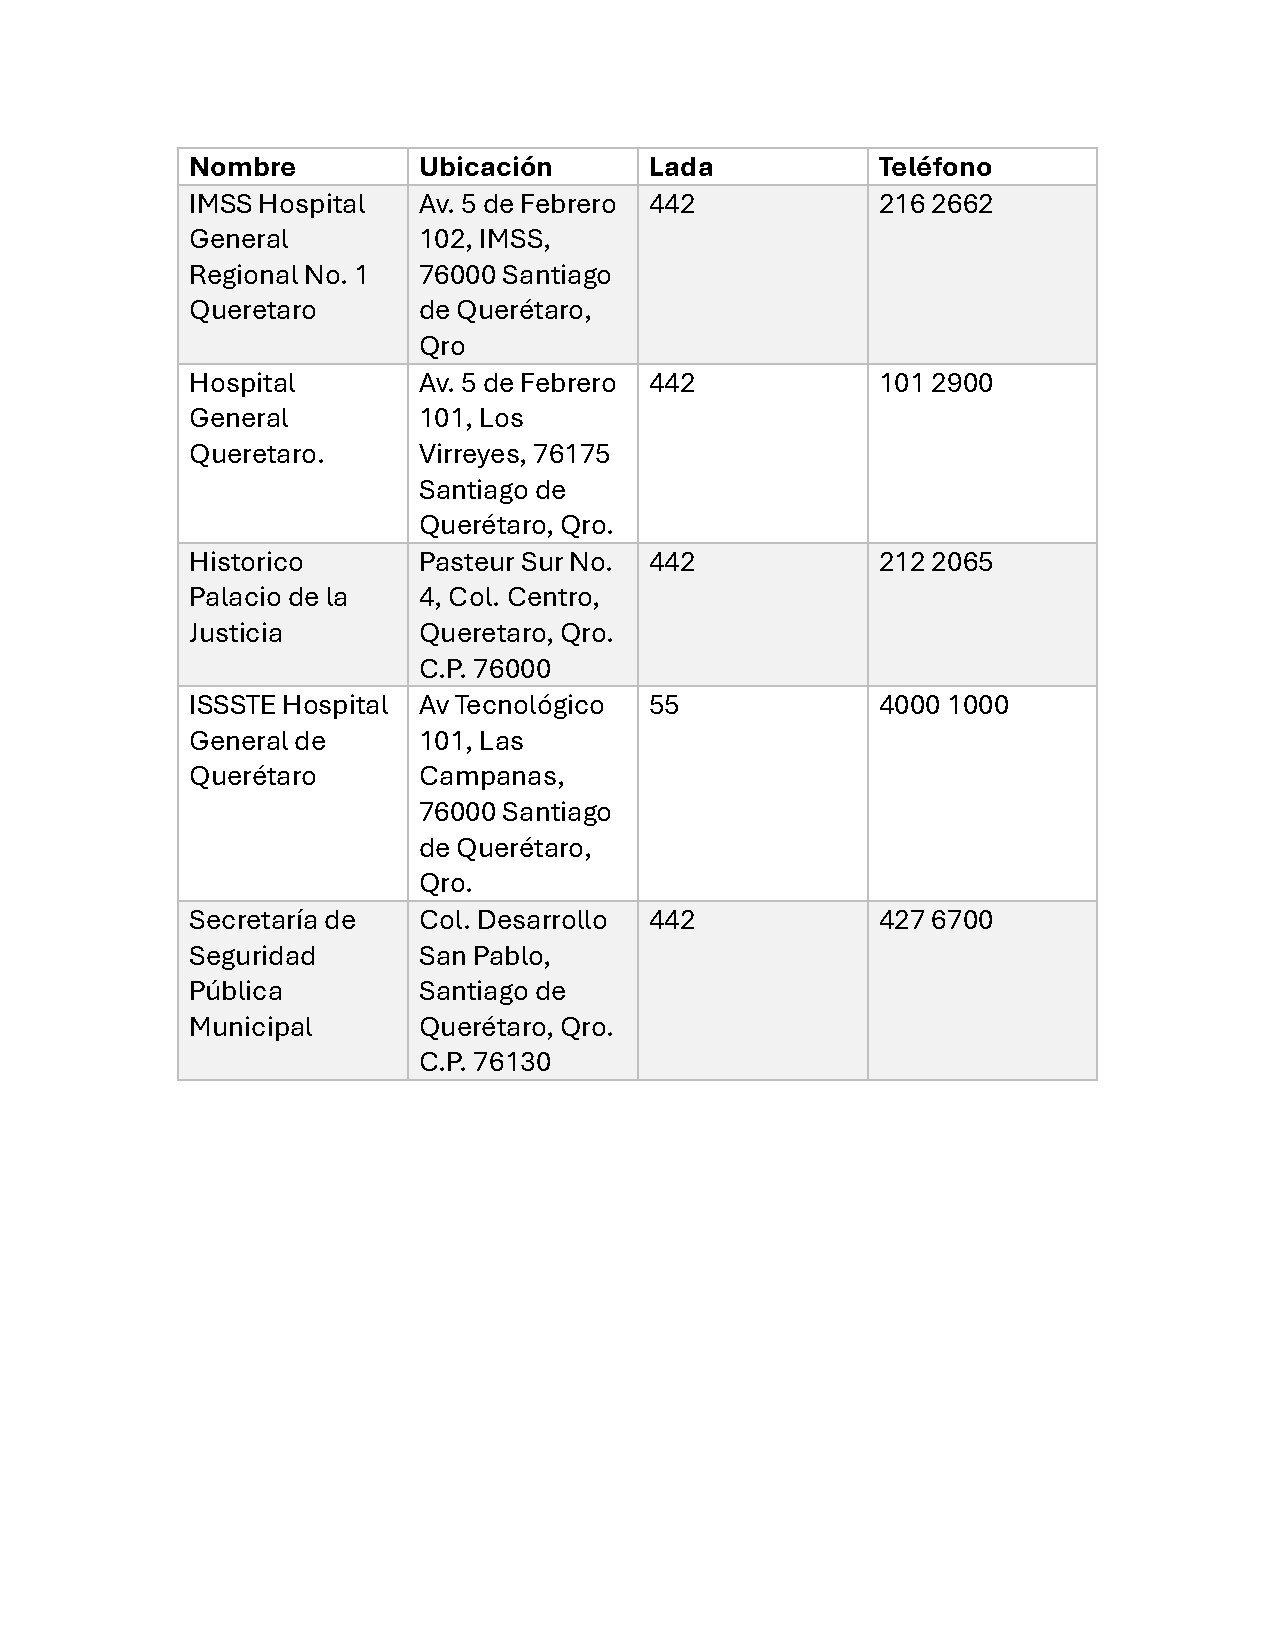
\includegraphics[trim = {20mm 95mm 20mm 41mm},clip,scale=0.5]{29/img/apoyosExternos.pdf}
        \caption{ Lugares que servirán de apoyo en un situación de emergencia.}
        \label{fig:apoyosExternos.pd}
    \end{figure}
    % 
    % 
    \subsubsection{Identificación de puntos de reunión}
    
    \begin{figure}[H]
        \centering
        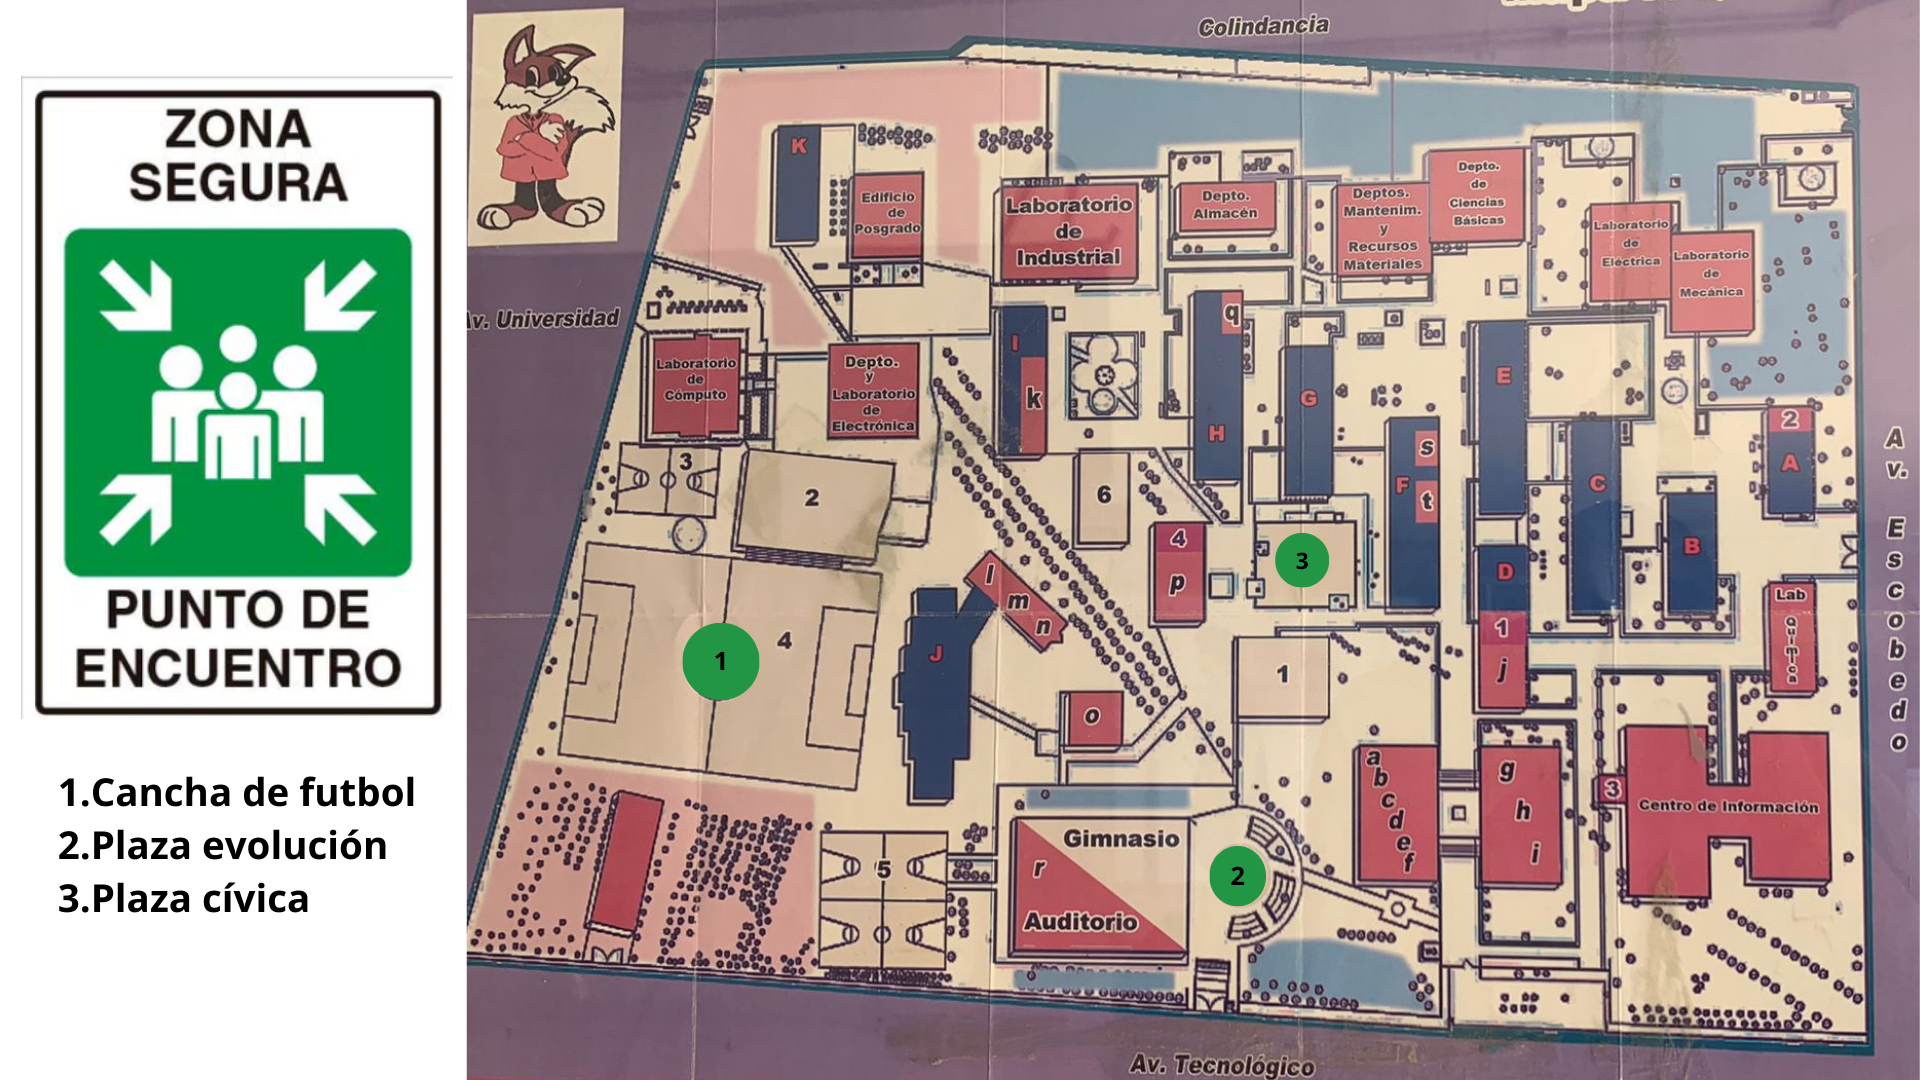
\includegraphics[trim = {40mm 60mm 20mm 21mm},clip,scale=0.35]{29/img/puntosDeReunion.pdf}
        \caption{Zona segura en caso de una evacuación de emergencia.}
        \label{fig:puntosDeReunion.pdf}
    \end{figure}
    % 
    % 
    \subsubsection{Brigada de evacuación}
    
    \begin{figure}[H]
        \centering
        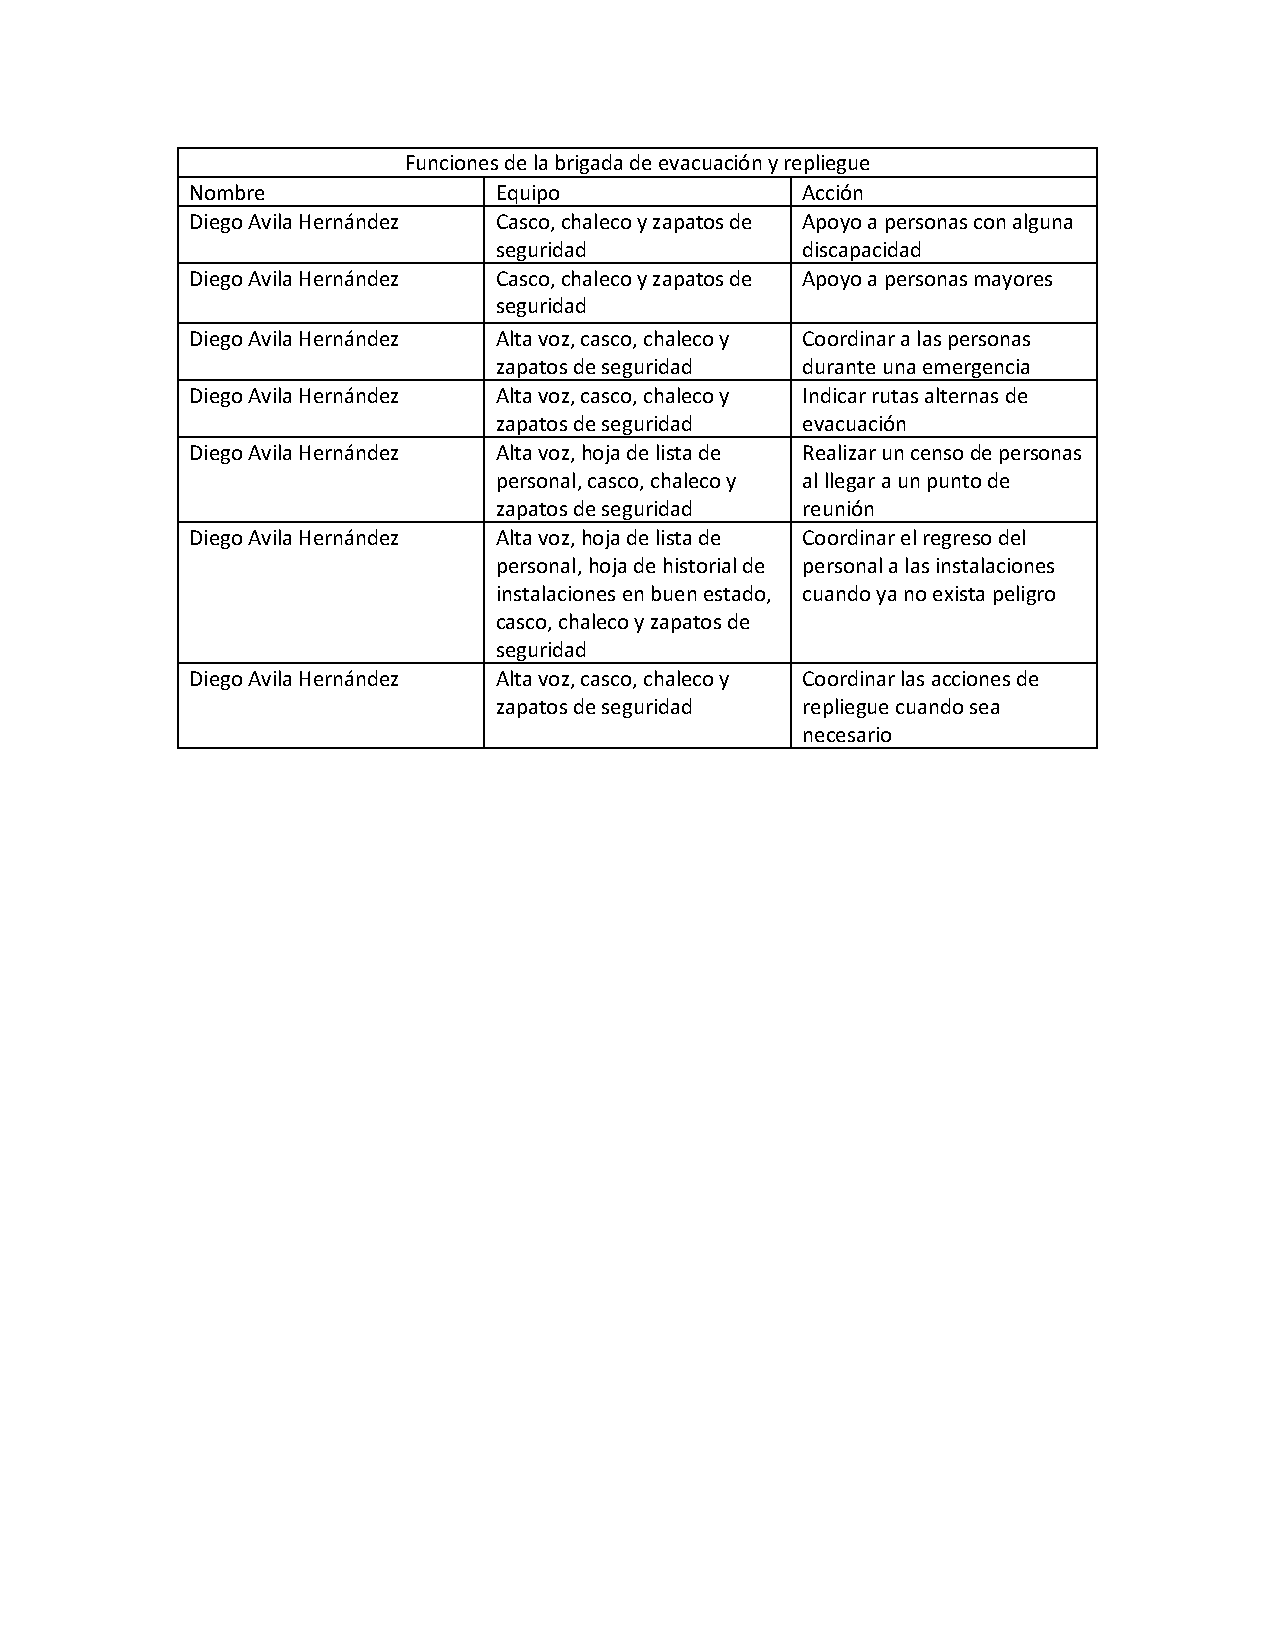
\includegraphics[trim = {20mm 90mm 40mm 45mm},clip,scale=0.5]{29/img/brigada.pdf}
        \caption{Acciones asignadas a cada integrante del equipo de trabajo en caso de una evacuación de emergencia o repliegue.}
        \label{fig:brigada.pdf}
    \end{figure}
    % 
    % 
    \subsubsection{Directorio de telefónicos de emergencia}
    
    Listado telefónico de instituciones de atención de emergencias y otras instituciones que intervengan para el seguimiento y control de las mismas.Identificar  lugares que servirán de apoyo en una situación de emergencia como clínicas, hospitales, módulos de guarida municipal, área de seguridad privada, mencionando, nombre de la institución, domicilio, teléfono, y servicios que ofrece. 
    
    \begin{figure}[H]
        \centering
        \includegraphics[scale=0.25]{29/img/bomberosEmergencia.pdf}
        \caption{Números de emergencia de los bomberos más próximos a la ubicación el posible riesgo}
    \end{figure}
    % 
    % 
    \begin{figure}[H]
        \centering
        \includegraphics[scale=0.45]{29/img/directorioEmergencias.pdf}
        \caption{Números de emergencia de los bomberos más próximos a la ubicación el posible riesgo}
    \end{figure}
    % 
    % 
    \subsection{Análisis de los métodos, materiales, herramientas e instalación utilizada en la ejecución del ensamble de un circuito electrónico}
    
    \subsubsection{Verificación}
    
    Costos de no calidad.
    % 
    % 
    \subsubsection{Desarrollo del sistema de tiempos predeterminado}
    En base al MTM-1 obtuvimos resultados los cual se registaron en una hoja de registro basándonos en el dato de la cantidad de movimientos y los pasos en los que se dividió el ensamble.
    \begin{figure}[H]
        \centering
        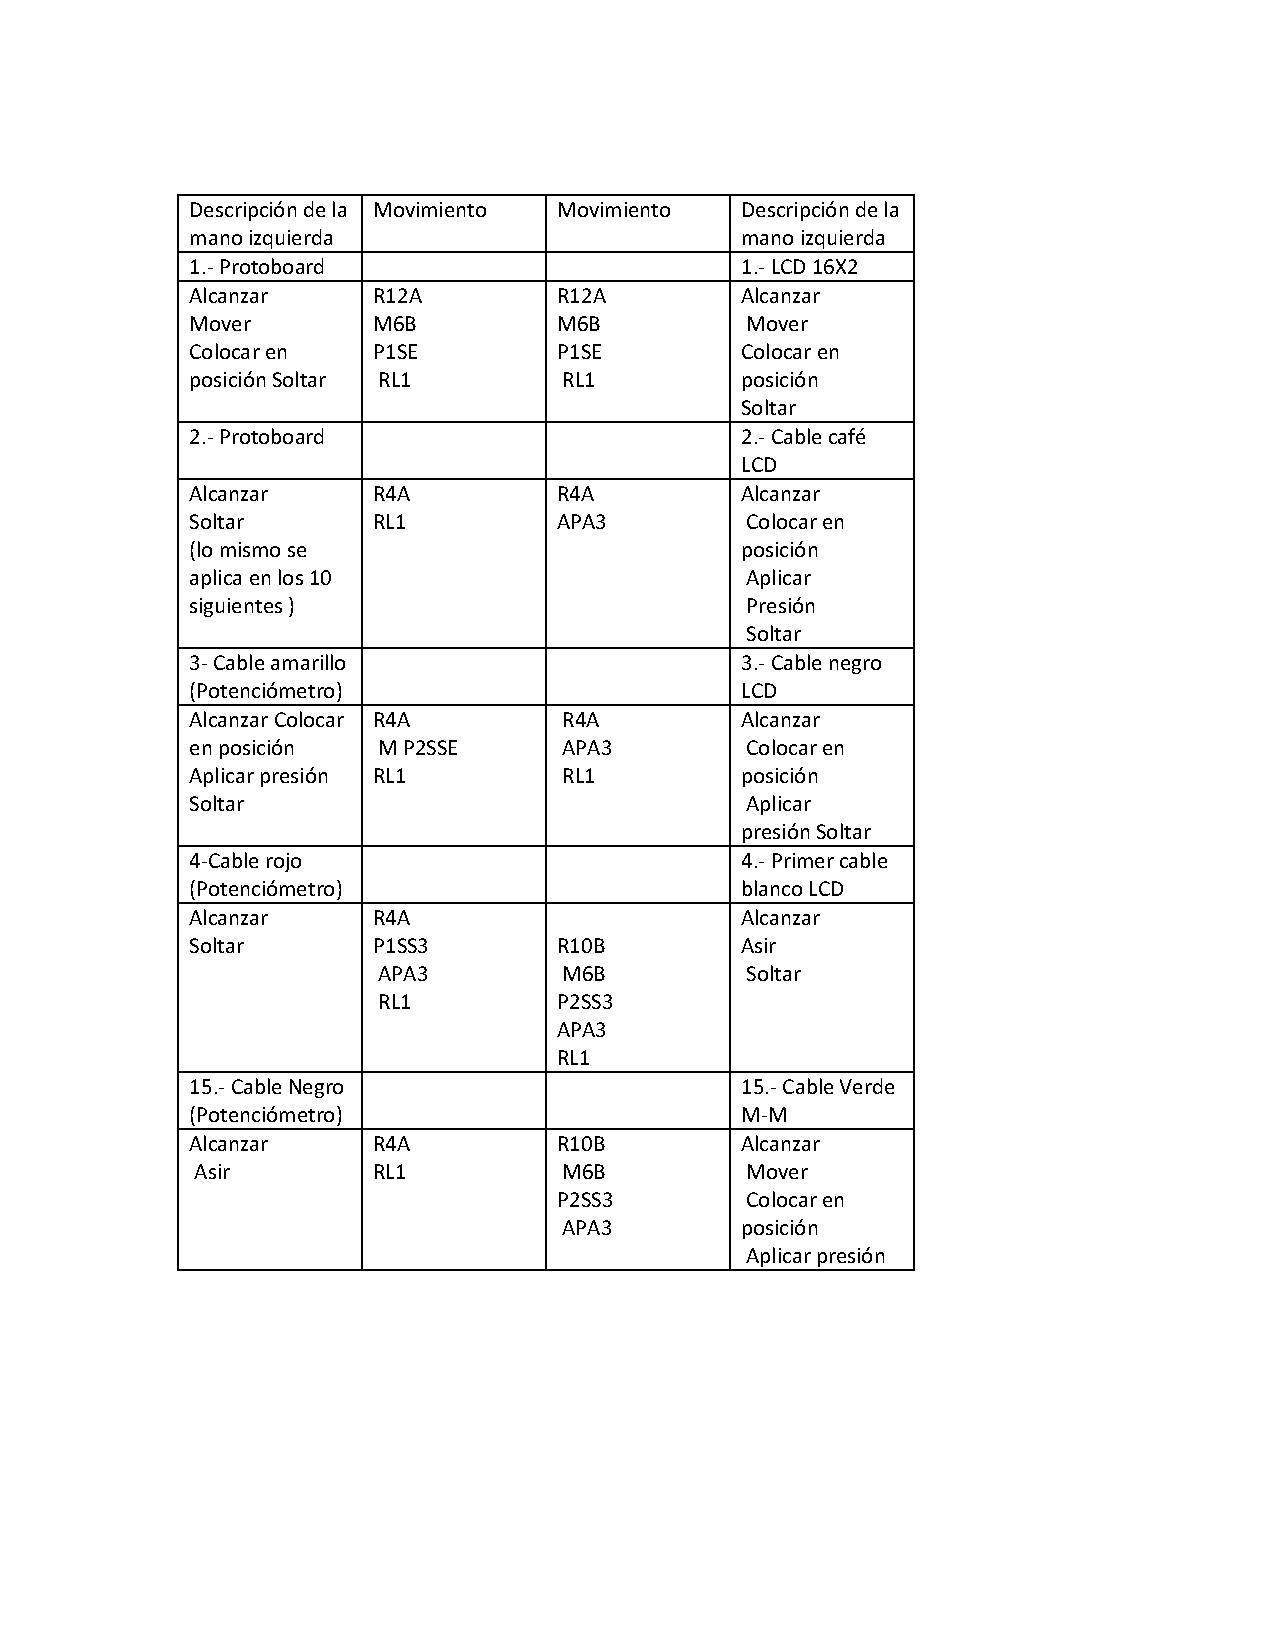
\includegraphics[scale=0.40]{29/img/tiemposPredeterminado.pdf}
        \caption{tiempo predeterminados  }
        \label{fig:tiemposPredeterminado.pdf}
    \end{figure}
    % 
    % 
    \subsubsection{Desarrollo del muestreo del trabajo}
    % 
    % 
    \subsubsection{Corrección por balanceo de procesos}
    % 
    % 
    \subsubsection{Datos estándar continuos y discretos}
    % 
    % 
    \subsection{Diseño de la forma más económica de realizar el trabajo}
    
    % 
    % 
    \subsection{Normalización de los métodos, materiales, herramientas e instalaciones}
    
    % 
    % 
    \subsection{Determinación del tiempo estándar para que una persona competente realice el trabajo con marcha normal}
    
    
    % 
    % 
    \section{Conclusiones}
    
    Se describe aquí el alcance del trabajo, logros obtenidos y perspectivas para el futuro de este. Se sugiere colocar información cuantitativa obtenida.
    
    \section{Agradecimientos}
    
    Es importante darles su debido reconocimiento a los laboratorios, instituciones, organizaciones, entre otros que han sido participes para la culminación de este trabajo. También es importante mencionar, fondos, proyectos, becas, entre otros que se le han otorgado al o los autores para realizar el trabajo de investigación. Ejemplo: “Los autores agradecen al Concejo Nacional de Ciencia y Tecnología por los recursos otorgados…”
    
    % \section*{Referencias}
    
    % Para esta platilla, se solicita al autor enumerar las citas de manera consecutiva entre corchetes \cite{YLi2013}. 
    % La puntuación de la oración que sigues sería \cite{Mesaelides2011}. 
    % Refiérase simplemente al número de referencia, como en \cite{Morales2012}, no utilice “Ref. [3]” o “referencia [3]” excepto al principio de una oración: “La referencia [3] fue la primera…”
    % Enumere las notas al pie por separado en superíndices. Coloque la nota de pie de en la parte inferior de la columna en la que se citó. No coloque notas al pie en la lista de referencias. Utilice letras para las notas al pie de la tabla.
    % A menos de que haya tres autores o más; no utilice “et al.”. Los trabajos que no hayan sido publicados, incluso si han sido presentados para su publicación, deben ser citados como “inéditos”. Los trabajos que han sido aceptados para su publicación deben de citarse como “en prensa”. Poner en mayúscula sólo la primera palabra de un título, excepto los nombres propios y los símbolos de elemento. 
    % Otros ejemplos \cite{LAAngeles2021}, \cite{LAAngelesConni}. 
    % Véase el link \cite{prueba}, Véase el Apéndice \ref{anexo:pines}.
    
    % Ejemplo
    %  @Article{article,
    % 	author = "Author1 LastName1 and Author2 LastName2 and Author3 LastName3",
    % 	title = "Article Title",
    % 	volume = "30",
    % 	number = "30",
    % 	pages = "10127-10134",
    % 	year = "2013",
    % 	doi = "10.3389/fnins.2013.12345",
    % 	URL = "http://www.frontiersin.org/Journal/10.3389/fnins.2013.12345/abstract",
    % 	journal = "Frontiers in Neuroscience"
    % }
    
    % @book{book,
    %   author    = {Author Name}, 
    %   title     = {The title of the work},
    %   publisher = {The name of the publisher},
    %   address   = {The city},
    %   year      = 1993,
    % }
    
    % @incollection{chapter,
    %   author       = {Bauthor Surname}, 
    %   title        = {The title of the work},
    %   editor       = {Editor Name},
    %   booktitle    = {The title of the book},
    %   publisher    = {The name of the publisher},
    %   address      = {The city},
    %   year         = 2002,
    %   pages        = {201-213},
    % }
    
    % @InProceedings{conference,
    %   author = {Cauthor Name and Dauthor Surname and Fauthor LastName},
    %   title = {The title of the work},
    %   booktitle = {The title of the conference proceedings},
    %   year = 1996,
    %   publisher = {The name of the publisher},
    %   editor = {Editor Name1 and Editor Name2},
    %   pages = {41-50},
    % }
    
    % @book{cho,
    %   author       = {Gauthor Name1}, 
    %   title        = {The title of the work},
    %   publisher = {Country code and patent number},
    %   address      = {Patent Country},
    %   year = 2013
    % }
    
    % @book{patent,
    %   author    = {Hauthor Surname1}, 
    %   title     = {The title of the work},
    %   publisher = {Patent number},
    %   address   = {Patent country},
    %   year      = 2010,
    % }
    
    % % please use misc for datasets
    % @misc{dataset, 
    % 	author = "Author1 LastName1 and Author2 LastName2 and Author3 LastName3",
    % 	title = "Data Title",
    % 	year = "2011",
    % 	doi = "10.000/55555",
    % 	URL = "http://www.frontiersin.org/",
    % }
    
    \bibliographystyle{ieeetr}
    \bibliography{6/referencias}
    % 
    % 
    %%%%%%%%%%%%%%%%%%%%%%%%%%%%%%%%%%
    \appendix
    %%%%%%%%%%%%%%%%%%%%%%%%%%%%%%%%%%
    % 
    % 
    % \centering{\section[\appendixautorefname{}]{Apéndice}}\label{anexo:pines}
    % \includepdf[pages=-]{6/Img/pines.pdf}
    %%%%%%%%%%%%%%%%%%%%%%%%%%%%%%%%%%%%%%%%